\documentclass[a4paper, titlepage, twoside]{article}
\usepackage{fancyvrb}
\usepackage{fancyhdr}
\usepackage{graphicx}
\newcommand{\qidl}{{\tt qidl}}
\newcommand{\codapi}{{\tt cod\_api}}
\newcommand{\idlgen}{{\tt idl\_gen}}
\newcommand{\master}{{\tt Codine::Master}}
\newcommand{\job}{{\tt Codine::Job}}
\newcommand{\queue}{{\tt Codine::Queue}}
\newcommand{\complex}{{\tt Codine::Complex}}
\newcommand{\calendar}{{\tt Codine::Calendar}}
\newcommand{\codine}{\textsc{Codine}}
\newcommand{\GRD}{\textsc{GRD}}

\begin{document}
\title{\Huge\bf Internship Report \\ \Large Summer Term 1999}
\author{Achim Demelt \\ University of Applied Sciences, Regensburg}
\date{\today}

\maketitle
\cleardoublepage
\tableofcontents
\vfill
\listoffigures
\cleardoublepage

\pagestyle{fancy}

\section{\label{s_intro}Introduction}
This report describes the main activity during my internship at Genias
Software GmbH, Neutraubling: provision of a CORBA
interface for Genias' load balancing software \textsl{\codine}, called 
\qidl. The following
two subsections give a brief overview of \codine\ and its migration to the
OO-world. Sections \ref{s_userdoc} and \ref{s_progdoc} will then reveal more
details about how to use \qidl\ and its technological background.

\textbf{Note:} Since most of this report will be reused as internal and 
external documentation for \qidl, it is written in English---according 
to guidelines at Genias.

\subsection{\label{s_Codine}Codine}
\codine\ is a workload management tool for heterogeneous, distributed computing
environments. It queues and executes batch jobs, thereby controlling the use
of shared resources to best achieve an enterprise's goals.

The \textsl{Global Resource Director (\GRD)}---based on \codine---provides
additional features, such as dynamic scheduling and fine-grained policy
definition and control. Although \GRD\ is a standalone product, the two terms
\textsl{\codine} and \textsl{\GRD}\ are used synonymously in this report. \qidl\
covers the whole range of \GRD\ functionality.

The basic principle of \codine\ is very simple: The user puts jobs with special
resource requirements (e.g. host architecture, memory requirements, software
licenses) into the system. \codine\ then tries to find a suitable place (called
\textsl{queue} in \codine\ terms) to run this job. If not enough resources can
be allocated, \codine\  holds the job back until resources become available
again.

The system administrator is offered many ways to configure the computing
cluster and to grant and deny access to parts of it to certain users and
user groups, depending on dynamically evaluated criteria. A detailed
explanation of all \codine/\GRD\ features cannot be given in this report (see
the \codine/\GRD\ user and administrator documentations
\cite{b_codine, b_grd} for more details), but
the reader should be familiar with the following terms:

\begin{description}
\item[Job:] A job is a computation task that a user wants to have executed on 
some machine in the computing cluster, e.g. a crash simulation in the automobile
industry or the flow of air around the wing of a plane. The user does not
care on \emph{which} machine his or her job is executed (especially when
there are several similar machines in the cluster), unless a minimum of
resource requirements are met (e.g. at least four processors, 512 MB of
RAM, and the simulation software available).

\item[Queue:] This is the place where a job can potentially run. A queue is
assigned to an \textsl{execution host} and offers a set of resources,
configured by the administrator. \codine\
matches the resources requested by a job with those offered by the
various queues and eventually schedules a job on an appropriate queue.

\item[Complex:] A complex is a set of attributes that describe a queue, a
host, or the computing capacities of a machine. Jobs may request these
attributes and the \codine\ scheduler then determines the appropriate queues.

\item[Users:] \GRD\ has four kinds of users: Managers, Operators, Owners, and
Users. Managers can manipulate all aspects of \GRD, operators are like managers
without permission of configuration changes,
owners may manipulate the queues or jobs they own, and users may 
submit and control their own jobs.

\item[Hosts:] Among the five types of hosts known to \GRD, only two are
relevant in this context: \textsl{Execution hosts}, where batch jobs are
executed, and the \textsl{master host}, where the \codine\ master daemon and
its job scheduler are
running on. An execution host can have more than one queue, whereas a queue
is associated with exactly one execution host.

\end{description}


\subsection{\label{s_corba}CORBA}
Following the trend towards object-orientation, \codine\ is to present itself in
an object-oriented manner. Up to its present release (4.2), \codine\ is written
entirely in C, thus ensuring high portability across various platforms.
Moreover, it offers a C programmer's interface (called \texttt{cod\_api}),
based on the \textsl{cull} (Common Usable List Library, \cite{b_cull}), 
a general-purpose doubly-linked
list written by Genias. It is therefore not feasible to change the complete
\codine\ kernel.

Due to increasing demands from the industry and engagement in several
projects sponsored by the German and European governments, Genias decided to
make the \codine\ functionality accessible via object-oriented interfaces
written in CORBA IDL. Since CORBA is an open standard and widely used in the
UNIX domain, it is regarded to be the best choice as a platform independent
environment.

One goal of \qidl\ was to keep very close to \codine's internal structures.
This simplifies the transition for a \texttt{cod\_api} programmer from the C-
to the CORBA-interface, since he or she will find familiar terms and
concepts---only a bit "objectized". But the real advantage lies at the
implementation side, where most of the basic CORBA server functionality can
be generated automatically out of existing C source code. Section
\ref{s_prog_idlgen} will focus on this topic in more detail. The following
section will explain the user's view of \codine's OO-face.

\cleardoublepage
\section{\label{s_userdoc}\qidl\---From the User's Perspective}
% supposed to be included by another LaTeX document

\subsection{Basic Concepts}
\qidl\ implements a set of CORBA interfaces for \codine/\GRD. These interfaces
allow access to all \GRD\ functionality as an alternative to the \codapi\ C
interface. It offers an object-oriented view of the \GRD\ system, with objects
like Master, Queue and Job. To provide a high degree of consistency and allow
an easy transition from \codapi\ to \qidl, the interfaces 
are closely related to their \codapi\ counterparts (i.e. cull lists).

This section describes the basic \qidl\ features on a more abstract and
informative level, whereas section \ref{s_user_using_qidl} applies and
describes these concepts in several examples. Section \ref{s_user_events} then
introduces the event facility of \qidl, which is used in the examples of
section \ref{s_user_using_qidl_rev}.

\subsubsection{\label{s_user_objects}The Objects}
Objects have been around in \codine\ for quite a long time, but have not been
implemented in an object oriented programming language. Instead, the
\codine\ objects were (and internally still are) represented
by their cull lists. The fields of a list element are so-to-speak the
object's attributes. Unfortunately, cull lists neither distinguish between
private and public fields, nor is there a notion of read-only attributes.
So much for encapsulation.

The operations on these cull "objects" are sparse: get, add, delete, and
modify. At least some relational database-like functionality is offered with
some sort of restriction and projection. Obviously this isn't what
object-orientation is all about.

A thorough examination of \codine's cull lists reveals the following objects,
represented here by their corresponding interfaces:

\begin{Verbatim}[fontsize=\small, frame=single]
module Codine
{
   interface Master;
   interface Queue;
   interface Job;
   interface Complex;
   interface Exechost;
   interface Checkpoint;
   interface ParallelEnvironment;
   interface UserProject;
   interface UserSet;
   interface Configuration;
   interface SchedConf;
   interface ShareTreeNode;
   interface Calendar;
};
\end{Verbatim}

The very first of these interfaces (\master) is the entry point for a \qidl\
client. There is exactly one object of this type for each \codine\ 
cell.\footnote{A \textsl{cell} is the part of the computing cluster that is
controlled by \codine.} 
Its object reference is made public and can be acquired by the client (see
section \ref{s_user_connecting}). This interface offers functions to
obtain the references of all other objects---the well-known jobs, queues,
complexes, and others. \codapi\ programmers might notice the similarities
between these interfaces and the \texttt{COD\_QUEUE\_LIST}, 
\texttt{COD\_JOB\_LIST}, and other macros from the C api.

Administration hosts, submit hosts, managers, and operators
are not represented as seperate interfaces. The simplicity of these "objects"
make this superfluous. They are handled as simple string lists.
All other objects' interfaces are embedded in a namespace called
\texttt{Codine} to avoid naming conflicts.

Once the client has acquired the desired objects, it can query all public
information about them, as well as navigate to all related objects, e.g.
from a queue to its attached complexes. Given the appropriate privileges, a
client can also create, delete, or modify objects. 

Since \codine\ is a multi-user system, an object can be deleted at any time,
either because of an explicit deletion request by an authorized user, or
naturally, e.g. by the completion of a job. So all \codine\ objects are highly
volatile---an object reference my become invalid any time. A client must
always be prepared to handle this situation. It is guaranteed, though, that
throughout the lifetime of a \emph{\codine}\ object, its corresponding CORBA
object will have the same object reference, unless the \qidl\ server is shut
down and restarted again.

\subsubsection{\label{s_user_connecting}Connecting the Server}
For a client program to interact with \qidl, it must acquire a reference to the
\master\ object, from which it can navigate to all other objects
such as queues and complexes. This reference is available via:
\begin{itemize}
\item A stringified version in
\texttt{\$CODINE\_ROOT/<cell>/common/master.ior}
\item Name service, under \texttt{/<cell>/Master} (optionally)
\item Environment variable (\texttt{\$CODINE\_MASTER\_IOR}, if set)
\end{itemize}
The safest way to connect the server is the first one, since the naming
service might crash or be manipulated otherwise, or the environment variable 
might not be set in the client process' environment. If, on the other hand, the
\texttt{\$CODINE\_ROOT} path is not accessible by the client, the other two
options are preferable.

\subsubsection{\label{s_user_authentication}Authentication}
In a standard CORBA 2.0 compliant environment, the server does not know,
where a request comes from. The IIOP layer must of course know the sender's
IP address, in order to send a reply, but it is not handed down to the
server's implementation code. The client's identity (i.e. user and group id's)
gets lost completely on the way.

This poses serious problems to \codine's access control concepts of managers,
operators, owners, and users, as well as its distinction of administration and 
submit hosts. It is
therefore necessary to provide a proprietary means of authentication, which
must be both easy to use and flexible enough to be extended in the future.
The CORBA concept of \textsl{contexts} seemds to be well suited for the
implementation of such a security framework.

CORBA contexts are a rarely used feature to send name/value pairs along with
a request. For the authentication problem, there is a context called
\texttt{cod\_auth}, whose value contains an encrypted string with some
information about the calling process. This string is usually generated by a
special library call, or granted by a trusted authority. 

All \qidl\ method signatures look like this:
\begin{Verbatim}[fontsize=\small, frame=single]
module Codine {
   interface Master {
      // ...
      QueueSeq    getQueues() context("cod_auth");
      // ...
   };
};
\end{Verbatim}
The actual value of the \texttt{cod\_auth} context is of no importance to
the user. It can contain anything from simple user identification to X.509
certificates or AFS tokens, as long as it is something that can be
decoded by \codine.

\subsubsection{\label{s_user_exceptions}Exceptions}
A client must be prepared to
handle an unexpected situation---exceptions in CORBA terms. \qidl\ defines
the following three exceptions:
\begin{Verbatim}[fontsize=\small, frame=single]
module Codine {
   // Answer thrown in case of an error
   struct Answer {
      cod_ulong   status;
      cod_string  text;
   };
   typedef sequence<Answer>   AnswerSeq;

   // Common Exceptions
   exception ObjDestroyed() {};
   exception Authentication {};
   exception Error {
      AnswerSeq   answer;
   };
};
\end{Verbatim}
\begin{description}
\item[ObjDestroyed:] This exception is thrown whenever the object that the
operation was called upon no longer exists. There is a subtle difference
between this and the standard \texttt{CORBA::INV\_OBJEREF} exception, which
means that the \emph{CORBA} object no longer exists.
\texttt{Codine::ObjDestroyed} means that the \emph{\codine}\ object no longer
exists.

\begin{figure}
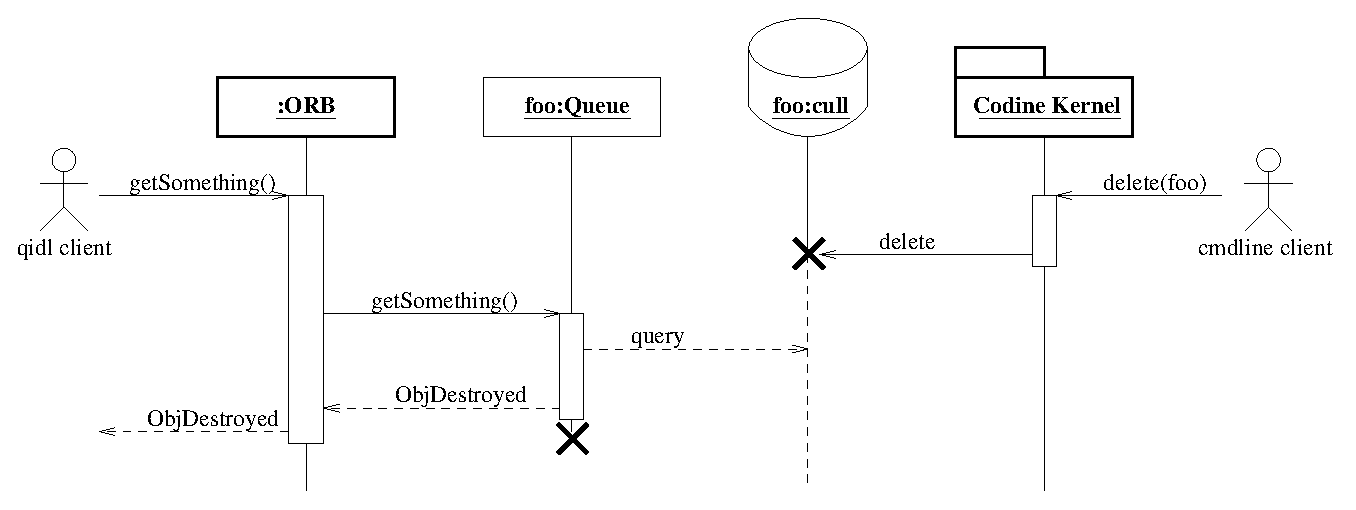
\includegraphics[width=\textwidth]{objdestroyed.eps}
\caption{\label{f_ObjDestroyed}The \texttt{Codine::ObjDestroyed} exception}
\end{figure}

Consider the situation in figure \ref{f_ObjDestroyed}. \qidl\
is a multithreaded server, so while the CORBA client's method is unmarshaled
and dispatched by the ORB (the CORBA object obviously still exists), a
command line client can delete the underlying \codine\ object. So the ORB
cannot and must not throw a \texttt{CORBA::INV\_OBJREF} exception, since
there is no reason to do so. Instead, \qidl\ notices that there is no longer
such an object and throws \texttt{Codine::ObjDestroyed}.

\item[Authentication:] As its name implies, this exception is thrown in case
of an authentication failure. Whenever there is an invalid or insufficient
\texttt{cod\_auth} context string assoiated with the operation, the client
will receive this error.

\item[Error:] Every \codapi\ call returns a so-called \textsl{answer list}.
This is a special-purpose cull list, that contains error messages and/or
warnings in case of failure, or simply a confirmation string. The
\texttt{AnswerSeq} above is the \qidl\ counterpart of the \codapi\ answer
list. The major difference between the two is that the \qidl\
\texttt{Codine::Error} exception (which contains the AnswerSeq), is only
thrown in case of an error. A \qidl\ client does not receive warnings and
confirmative messages.
\end{description}

\subsubsection{Data Retrieval and Manipulation}
After connecting to the server, considering authentication and exception
handling, a client will want to request information from \codine\ 
and add or modify data. For this purpose, \qidl\ offers a rich IDL
interface for its objects, tightly coupled with their underlying cull lists.

The first step is to retrieve references to the desired objects from the
master. The \master\ interface provides the following functions (excerpt):

\begin{Verbatim}[fontsize=\small, frame=single]
module Codine {
   interface Master : CosEventComm::PushSupplier {
      // object retrieval
      QueueSeq          getQueues() context("cod_auth");
      JobSeq            getJobs() context("cod_auth");
      ComplexSeq        getComplexes() context("cod_auth");
      ConfigurationSeq  getConfigurations() context("cod_auth");
      CalendarSeq       getCalendars() context("cod_auth");
      CheckpointSeq     getCheckpoints() context("cod_auth");
      UserSetSeq        getUserSets() context ("cod_auth");
      // ...
   };
};
\end{Verbatim}

For each class of objects, there is a corresponding \texttt{getXXXs()} method
that returns a sequence of all currently available objects of that
type.\footnote{These functions return a list of object \emph{references}, not
the object themselves, which is standard CORBA behavior.}
The client can traverse the sequence and invoke operations directly on the
contained objects, e.g. a queue (excerpt):

\begin{Verbatim}[fontsize=\small, frame=single]
module Codine {
   interface Queue : Codine::Obj {
      cod_string get_qname()
            raises(ObjDestroyed, Authentication, Error)
            context("cod_auth");
      cod_string get_qhostname()
            raises(ObjDestroyed, Authentication, Error)
            context("cod_auth");
      cod_ulong set_qhostname(in cod_string val) 
            raises(ObjDestroyed, Authentication, Error) 
            context("cod_auth");
      cod_ulong get_seq_no() 
            raises(ObjDestroyed, Authentication, Error) 
            context("cod_auth");
      cod_ulong set_seq_no(in cod_ulong val) 
            raises(ObjDestroyed, Authentication, Error) 
            context("cod_auth");
      ComplexEntrySeq get_load_thresholds() 
            raises(ObjDestroyed, Authentication, Error) 
            context("cod_auth");
      cod_ulong set_load_thresholds(in ComplexEntrySeq val) 
            raises(ObjDestroyed, Authentication, Error) 
            context("cod_auth");
      Calendar get_calendar() 
            raises(ObjDestroyed, Authentication, Error) 
            context("cod_auth");
      cod_ulong set_calendar(in Calendar val) 
            raises(ObjDestroyed, Authentication, Error) 
            context("cod_auth");
      ComplexSeq get_complex_list() 
            raises(ObjDestroyed, Authentication, Error) 
            context("cod_auth");
      cod_ulong set_complex_list(in ComplexSeq val) 
            raises(ObjDestroyed, Authentication, Error) 
            context("cod_auth");
      // ...
   };
};
\end{Verbatim}

To underline the similarity to the queue's cull list, here's an excerpt from
the \codapi\ C header file:

\begin{Verbatim}[fontsize=\small, frame=single]
LISTDEF( QU_Type )
 COD_STRING( QU_qname )        /* name of Q                    */
 COD_STRING( QU_qhostname )    /* qualified hostname           */
 COD_ULONG( QU_seq_no )        /* sequence # for use by qmon   */
 COD_LIST( QU_load_thresholds )/*   list of load alarm values  */
 COD_STRING( QU_calendar )     /* name of the calendar or NULL */
 COD_LIST( QU_complex_list )   /* user defined queue complexes */
LISTEND
\end{Verbatim}

The cull fields are translated into IDL \texttt{get\_} and \texttt{set\_}
operations. Each of these functions can raise the exceptions explained in
section \ref{s_user_exceptions}, and requires the \texttt{cod\_auth} context.
This is also the reason why \qidl\ cannot use IDL attributes, since these
don't allow user-defined exceptions and contexts. The \texttt{set\_}
functions return an integer value which is used in the context of event
handling (see section \ref{s_user_events}). Otherwise it is of no use and can
be ignored.

Apart from functions for attributes with simple data types (e.g.
\texttt{get\-\_qhostname()}, \texttt{set\_seq\_no()}), there are three other
types of functions:

\begin{itemize}
\item Functions for attributes with compound types (i.e. structs, sequences of
structs)
\item Functions for attributes with object types (i.e. object references,
sequences of object references)
\item Miscellanous and "convenience" functions
\end{itemize}

\paragraph{Functions for Attributes with Compound Types\\}
\texttt{get/set\_load\_thresholds()} are examples for this
type of function. They provide access to the queue's load alarm values,
stored in a sequence of structs of type \texttt{Codine::ComplexEntry} which
is defined as follows:

\begin{Verbatim}[fontsize=\small, frame=single]
module Codine {
   struct ComplexEntry {
      cod_string name;
      cod_string shortcut;
      cod_ulong valtype;
      cod_string stringval;
      cod_ulong relop;
      cod_ulong request;
      cod_ulong consumable;
      cod_ulong forced;
   };
   typedef sequence<ComplexEntry> ComplexEntrySeq;
};
\end{Verbatim}

Again, this structure is a direct translation of the corresponding cull list
type. But since this is only a container for a set of data and no long-lived
object controlled by the master, it is not transformed into an interface, but
only into a struct. As the CORBA standard specifies, the sequence really
\emph{contains} these data structures, not only references to them.

\paragraph{Functions for Attributes with Object Types\\}
The last four functions of the \queue\ interface concern the links of a queue
to other objects; in this case to its associated \calendar\ and \complex\
objects. These functions take or return \emph{references} or a \emph{sequence
of references} to objects managed by \master.

Note that the queue's cull list identifies its calendar only with its name
(\texttt{COD\_STRING( QU\_calendar )}), whereas in \qidl\ it is a real object
reference. In addition, there is no distinction between object reference and
struct containment in the cull, as can be seen from the
\texttt{QU\_load\_thresholds} and \texttt{QU\_complex\_list} entries; both
are of type \texttt{COD\_LIST}. \qidl\
provides a far better distinction here and reflects the true nature of the
objects' structure and interconnections.

\paragraph{Miscellanous and Convenience Functions\\}
Creation and deletion of objects fall under this category. Convenience
functions are those that would otherwise require the manipulation of certain
attributes in a certain way, just to achieve one simple goal. This
includes functions to hold or suspend a job, among others. The following two
subsections describe these in more detail.

Every retrieval or manipulation of an object's data requires a seperate COR\-BA
request. Depending on the underlying software implementation and network
structure, this can pose serious performance problems to both the client and
the master. To overcome this, every object offers functions to retrieve or
manipulate the object's state in one single method invocation. These are
defined in a common base interface from which all other interfaces except
\master\ are derived:

\begin{Verbatim}[fontsize=\small, frame=single]
module Codine {
   // Content of an object as (name,value) pairs
   struct content {
      cod_ulong   elem;
      any         value;
   };
   typedef sequence<content> contentSeq;

   // THE base class
   interface Obj {
      // opaque object state
      contentSeq  get_content() 
            context("cod_auth");
      cod_ulong   set_content(in contentSeq state) 
            context("cod_auth");
      
      oneway void destroy() context("cod_auth");
   };
};
\end{Verbatim}

The \texttt{Codine::content} structure represents exactly one field of a cull
list element. It is identified by its unique element key (\texttt{elem}), and
its value of type \texttt{CORBA::any}. The element keys are defined as
constants with the same identifier as their corresponding entries in
the cull list definitions (e.g. \texttt{QU\_qhostname}). These constants can
be found in the file \texttt{elem\_codes.idl}, a small excerpt of which is shown
here:

\begin{Verbatim}[fontsize=\small, frame=single]
module Codine {
   const unsigned long JB_job_number = 50;
   const unsigned long JB_script_file = 53;
   const unsigned long JB_script_size = 54;
   const unsigned long JB_script_ptr = 55;
   const unsigned long JB_submission_time = 57;
   const unsigned long JB_start_time = 58;
   const unsigned long JB_end_time = 59;
   const unsigned long JB_owner = 60;
   const unsigned long JB_account = 75;
   const unsigned long JB_cell = 80;
   // ...
   const unsigned long QU_qname = 250;
   const unsigned long QU_qhostname = 251;
   const unsigned long QU_priority = 261;
   const unsigned long QU_qtype = 263;
   const unsigned long QU_processors = 264;
   const unsigned long QU_job_slots = 265;
   const unsigned long QU_prolog = 267;
   // ...
   const unsigned long EH_scaling_list = 451;
   const unsigned long EH_complex_list = 452;
   const unsigned long EH_consumable_config_list = 453;
   const unsigned long EH_usage_scaling_list = 454;
   const unsigned long EH_load_list = 455;
   const unsigned long HL_name = 700;
   const unsigned long HL_value = 701;
   const unsigned long HS_name = 750;
   const unsigned long HS_value = 751;
   // ...
};

\end{Verbatim}

An object's state can be completely described by this \texttt{contentSeq}, so
per\-formance-critical applications can and should use these functions to 
interact efficiently with \codine. A similar mechanism is used for event
handling, as described in section \ref{s_user_events}.

\subsubsection{Creating and Deleting Objects}
Deleting an object is fairly simple. Every \codine\ object presented in section
\ref{s_user_objects} is derived from a common base interface,
\texttt{Codine::Obj}, as shown in the previous subsection. Recall that apart
from the state functions it also defines a \texttt{oneway void destroy()}
method to delete the object. It's usage is straightforward; the called-upon 
object won't exist anymore, unless the calling process doesn't have the
necessary privileges to dispose it (e.g. a normal user must not delete a
queue, but is allowed to cancel the jobs he or she submitted).

Creating objects is \master's responsibility. Remember that all \codine\
objects are managed by the master, so this is the canonical instance to request
new objects from. There are corresponding functions to do so:

\begin{Verbatim}[fontsize=\small, frame=single]
module Codine {
   interface Master : CosEventComm::PushSupplier {
      // ...
      Queue          newQueue(in string name)
            context("cod_auth");
      Job            newJob() 
            context("cod_auth");
      Complex        newComplex(in string name)
            context("cod_auth");
      Configuration  newConfiguration(in string hname)
            context("cod_auth");
      Calendar       newCalendar(in string name)
            context("cod_auth");
      Checkpoint     newCheckpoint(in string name)
            context ("cod_auth");
      ParallelEnvironment newParallelEnvironment (in string name)
            context ("cod_auth");
      UserSet        newUserSet(in string name)
            context ("cod_auth");
      // ...
   };
};
\end{Verbatim}

These functions return a reference to the newly created object. This
object is \emph{not} yet publicly visible to any other \codine\ client except
the one that created it, since other users should not see 
objects currently in their creation process. To permanently save an object in
the master's database and thus making it available to other users,
each object provides a corresponding \texttt{add()} function (for jobs
this is naturally called \texttt{submit()}).

\subsubsection{\label{s_user_convenience}Convenience Functions}
Convenience functions encapsulate common manipulations of object states in
easy-to-use methods. The following paragraphs show and---if 
necessary---ex\-plain
these functions for each \codine\ object. Most of them return an integer value
for use with event handling (section \ref{s_user_events}).
Note that this feature is still under development and more are functions are
being added permanently.

\paragraph{Job}
\begin{Verbatim}[fontsize=\small, frame=single]
module Codine {
   interface Job : Codine::Obj {
      cod_ulong   hold() 
            raises(ObjDestroyed, Authentication, Error)
            context("cod_auth");
      cod_ulong   suspend(boolean force)
            raises(ObjDestroyed, Authentication, Error)
            context("cod_auth");
   };
};
\end{Verbatim}

\paragraph{Master}
\begin{Verbatim}[fontsize=\small, frame=single]
module Codine {
   interface Master : CosEventComm::PushSupplier {
      // ...
      boolean registerObject(in unsigned long jid,
                             in Object obj);
      boolean unregisterObject(in unsigned long jid, 
                             in Object obj);

      oneway void shutdown() context("cod_auth");
      // ...
   };
};
\end{Verbatim}
\begin{description}
\item[{[un]}registerObject:] These functions allow a \codine\ job that
implements any type of CORBA server to register with \qidl. \codine\ 
associates the given object's reference with its job id. Clients can query
this information from \codine\ and thus use it as some sort of CORBA name
service.\footnote{This is of course not a name service as specified by
the OMG, but a mere coupling of job id's and object references.} 
The implementation of this
function sets or unsets a special context tag (\texttt{IOR}) in the given 
jobs data structure. See the \codine\ User's Manual for more information about
job contexts.

These functions are included in the \master\ interface to provide a simple way
for code suppliers to integrate their product with \codine. By using this
function, they don't need to retrieve the job list, find their corresponding
job object, and modify this job's context sequence.

\item[shutdown:] This shuts down the \qidl\ server. Use this with caution.
\end{description}

\subsection{\label{s_user_using_qidl}Using \qidl}
This section contains detailed code examples that show how to use \qidl\ as a
client. Section \ref{s_user_using_common} describes the common tasks that
each client has to perform in order to communicate with the \qidl\ server.
For brevity and to avoid repetition, these tasks will be omitted in the
following subsections, which highlight some common uses of \qidl. Note
that the presented examples were written using OOC's \textsl{ORBacus} CORBA
implementation. Some modifications might be necessary for use with other
ORBs, expecially concerning namespace/module support (\texttt{::} syntax
instead of \texttt{\_}).

\subsubsection{\label{s_user_using_common}Common Tasks}
Each \qidl\ client must obey to certain rules in order to establish and
maintain a stable connection to the \qidl\ server. These are:
\begin{enumerate}
\item Initialize the ORB
\item Acquire the server's object reference
\item Acquire a valid authentication string
\item Create a CORBA context object
\item Pass this context with all method invocations
\item \label{e_user_catch_exceptions}Always be prepared to catch an exception
\end{enumerate}
Initializing the ORB is vendor dependent and will not be explained further
here. For acquiring the server's object reference, a client can use any of
the three options described in section \ref{s_user_connecting}. We will use a
combination of all three in the following example. The authentication string
will come from a library function, and the creation of the CORBA context
object is standard CORBA 2.0 code.

\begin{Verbatim}[frame=lines, numbers=left, fontsize=\small, framerule=1mm]
// forward decls
CORBA_Object_ptr getMasterViaFile(CORBA_ORB_var& orb);
CORBA_Object_ptr getMasterViaNameService(CORBA_ORB_var& orb);
CORBA_Object_ptr getMasterViaEnv(CORBA_ORB_var& orb);

int main(int argc, char** argv) {
   try {
      CORBA_Object_var  obj;
      CORBA_ORB_var     orb;
      Codine_Master_var master;
      CORBA_any         any;
      CORBA_Context_ptr ctx;


      // initializing ORB...
      orb = CORBA_ORB_init(argc, argv);
      if(CORBA_is_nil(orb)) {
         cerr << "could not init ORB." << endl;
         return 1;
      }

      // trying to get the master's object reference
      obj = getMasterViaEnv(orb);
      if(CORBA_is_nil(obj))
         obj = getMasterViaNameService(orb);
      if(CORBA_is_nil(obj))
         obj = getMasterViaFile(orb);
      if(CORBA_is_nil(obj)) {
         cerr << "could not get master's object reference.";
         cerr << endl;
         return 1;
      }

      // narrow the object to the correct type
      master = Codine_Master::_narrow(obj);
      if(CORBA_is_nil(master)) {
         cerr << "could not narrow the object reference.";
         cerr << endl;
         return 1;
      }
      
      // create authentication context
      any <<= get_cod_auth();
      orb->get_default_context(ctx);
      ctx->set_one_value("cod_auth", any);

      // here comes the client code
      // ...
   }
   catch(CORBA_System_Exception& x) {
   }
   catch(Codine_ObjDestroyed& x) {
      cerr << "The object does no longer exist!" << endl;
   }
   catch(Codine_Error& x) {
      cerr << "Codine Error: " << endl;
      for(CORBA_ULong i=0; i<x.answer.length(); i++)
         cerr << x.answer[i].text;
   }
   catch(Codine_Authentication& x) {
      cerr << "Codine authentication problem!" << endl;
   }
   catch(...) {
      cerr << "Caught unknown exception!" << endl;
   }

   return 0;
}

CORBA_Object_ptr getMasterViaEnv(CORBA_ORB_var& orb) {
  if(getenv("CODINE_MASTER_IOR"))
    return orb->string_to_object(getenv("CODINE_MASTER_IOR"));
  else
    return CORBA_Object::_nil();
}

CORBA_Object_ptr getMasterViaNameService(CORBA_ORB_var& orb) {
   CORBA_Object_ptr obj = CORBA_Object::_nil();
   CORBA_Object_var ns_obj;
   CosNaming_NamingContext_var ns;
   CosNaming_Name_var name;

   try {
      ns_obj = orb->resolve_initial_references("NameService");
      if(CORBA_is_nil(ns_obj)) {
         cerr << "Don't have name service." << endl;
         return obj;
      }
      ns = CosNaming_NamingContext::_narrow(ns_obj);
      if(CORBA_is_nil(ns)) {
         cerr << "Not a name service." << endl;
         return obj;
      }
      name = new CosNaming_Name();
      name->length(2);
      name[0].id = CORBA_string_dup(getenv("CODINE_CELL")?
                         getenv("CODINE_CELL"):"default");
      name[0].kind = CORBA_string_dup("");
      name[1].id = CORBA_string_dup("cod_qidl");
      name[1].kind = CORBA_string_dup("");
   
      obj = ns->resolve(name);
   }
   catch(...) {
      cerr << "Problems with name service." << endl;
   }

   return obj;
}

CORBA_Object_ptr getMasterViaFile(CORBA_ORB_var& orb) {
   CORBA_Object_ptr obj = CORBA_Object::_nil();
   char ref[1024];
   char* croot = getenv("CODINE_ROOT");
   
   if (!croot) {
      cerr << "No CODINE_ROOT set." << endl;
      return obj;
   }
   string filename = croot;
   filename += "/default/common/master.ior";
   ifstream ref_file(filename.c_str());
   if(ref_file) 
      ref_file >> ref;
   ref_file.close();
   obj = orb -> string_to_object(ref);

   return obj;
}
\end{Verbatim}

Implementing the client's main routine is fairly straightforward considering
the rules mentioned above. After initializing the ORB in line 16, it tries to
retrieve the server's object reference by calling the three helper functions
(lines 22-40). In line 43, the client's authentication string (returned by
the library function \texttt{get\_cod\_auth()}) is pushed into a
\texttt{CORBA::Any} variable. The global CORBA context variable \texttt{ctx}
is initialized with the default context (line 44), and finally in line 45, the
\texttt{cod\_auth} entry is set as the context's only value. The actual
client code (not present in this example) can safely  use the \master\ object 
from this point.

All this code is encapsulated in a \texttt{try...catch} statement, according
to rule \ref{e_user_catch_exceptions} on page
\pageref{e_user_catch_exceptions}. Apart from the CORBA system exceptions and
other (unkown) exceptions, the three custom \qidl\ exceptions are handled
correctly (lines 50-65). Of course, the main program is not a good place to
seriously handle these exceptions, since no useful recovery is possible from
there. More fine-grained \texttt{try...catch} layers are necessary.

As mentioned before, the actual retrieval of the \qidl\ server's object
reference is done in three helper functions:

\begin{description}
\item[getMasterViaEnv:] The most trivial way to accomplish this task is to
read the \texttt{CODINE\_MASTER\_IOR} environment string and convert it to a
CORBA object reference with \texttt{CORBA::ORB.string\_to\_object()}.
\item[getMasterViaNameService:] This is a bit more complicated than the first
possibility. After successfully acquiring the name service object from the
ORB (lines 84-93), a naming context for the \qidl\ object is created in lines
94-100. Its reference is stored in \texttt{/<CODINE\_CELL>/cod\_qidl}.
\texttt{CODINE\_CELL} is the currently active cell (queried from the
corresponding environment variable), or the \texttt{default} cell. Line 102
then simply has to resolve the object from the name service.
\item[getMasterViaFile:] The safest way to retrieve the master object is to
read from the \texttt{\$CODINE\_ROOT/<cell>/common/master.ior} file, where
\codine\ writes the stringified object reference of the \qidl\ server. Lines
111-129 do right that, assuming the default cell as the currently active
\codine\ cell. \codine's root directory must of course be shared and 
read-accessible for the client process for this approach.
\end{description}

\subsubsection{Querying and Modifying Queue Attributes}
This subsection shows how to retrieve and modify
\begin{itemize}
\item simple attributes (i.e. those with a fundamental data type),
\item compound attributes (i.e those with a \texttt{struct} type), and
\item relations to other objects
\end{itemize}
of a queue. The example assumes that \codine\ is correctly installed and
running, there is at least one queue configured in the system, and all
initialization tasks as described in section \ref{s_user_using_common} 
have been performed successfully. No additional error and exception handling is
done here to keep the code more readable.
The code is executed inside a function which receives the \master\ object
reference and the context variable as parameters.

\begin{Verbatim}[frame=lines, numbers=left, fontsize=\small, framerule=1mm]
void query_mod_queue_attr(Codine_Master_ptr master,
                          CORBA_Context_ptr ctx) {
   // local variables
   CORBA_ULong                   i;
   Codine_QueueSeq_var           qs;
   Codine_Queue_var              q;
   
   // get the first queue from qmaster
   qs = master->getQueues(ctx);
   q = qs[0];                    // assume it exists

   // print out simple attributes
   cout << "QueueName: " << q->get_qname(ctx) << endl;
   cout << "on host  : " << q->get_qhostname(ctx) << endl;
   cout << "slots    : " << q->get_job_slots(ctx) << endl;
   
   // print out compound attributes
   Codine_ComplexEntrySeq_var lts;
   lts = q->get_load_thresholds(ctx);
   cout << "load thresholds:" << endl;
   for(i=0; i<lts->length(); i++) {
      cout << "   name: " << lts[i].name << endl;
      cout << "   valtype: " << lts[i].valtype << endl;
      cout << "   stringval: " << lts[i].stringval << endl;
      cout << "   ---------------------------------" << endl;
   }

   // print out relations to and contents of other objects
   Codine_ComplexSeq_var cs;
   cs = q->get_complex_list(ctx);
   cout << "attached complexes:" << endl;
   for(i=0; i<cs->length(); i++)
      cout << "   " << cs[i]->get_name(ctx) << endl;

   // modify slot number
   cout << endl << "Setting slots to 5...";
   q->set_job_slots(5, ctx);
   cout << "done." << endl;
   
   // delete load thresholds
   cout << "Removing any load thresholds...";
   lts->length(0);
   q->set_load_thresholds(lts, ctx);
   cout << "done." << endl;

   // checking modifications
   cout << endl << "Checking Modifications:" << endl;
   cout << "slots    : " << q->get_job_slots(ctx) << endl;
   lts = q->get_load_thresholds(ctx);
   if(lts->length() == 0)
      cout << "No load thresholds set." << endl;
   else
      cout << "Load thresholds still set!" << endl;
   
   // append a load threshold again
   cout << endl << "Appending a load threshold...";
   lts->length(1);
   lts[0].name = CORBA_string_dup("load_avg");
   lts[0].shortcut = CORBA_string_dup("");
   lts[0].valtype = 0;
   lts[0].stringval = CORBA_string_dup("175");
   lts[0].relop = 0;
   lts[0].request = 0;
   lts[0].consumable = 0;
   lts[0].forced = 0;
   q->set_load_thresholds(lts, ctx);
   cout << "done." << endl;

   // checking again
   cout << endl << "load thresholds now:" << endl;
   for(i=0; i<lts->length(); i++) {
      cout << "   name: " << lts[i].name << endl;
      cout << "   valtype: " << lts[i].valtype << endl;
      cout << "   stringval: " << lts[i].stringval << endl;
      cout << "   ---------------------------------" << endl;
   }
}
\end{Verbatim}

Lines 8-10 assign the first \codine\ queue in the list to the local variable
\texttt{q} (assuming there is at least one queue). Then, in lines 12-15,
three simple attributes are retrieved with their corresponding \texttt{get\_}
methods. Printing out compound attributes isn't much more complicated.
Querying the sequence of load thresholds (of type
\texttt{Codine::ComplexEntry}) and looping over its contents is performed in
lines 17-26. Note that the actual values of the sequence's contents are
\emph{not} retrieved with a function call, but with simple member access.

The queue's attached complexes are retrieved in line 30. This method returns
a sequence of object references to \complex es. Their names are printed out
in lines 31-33.

Changing attribute values is just as easy as reading them; calling the
\texttt{set\_} function is sufficient (lines 35-38). Lines 40-44 remove the
queue's load thresholds by setting the sequence length to zero (and thus
clearing it), and then setting the empty list as the new load threshold
sequence. Lines 46-53 simply check and display these changes.

Appending a load threshold (lines 55-67) is a bit more complicated, since a
complete \texttt{Codine::ComplexEntry} struct must be filled out correctly.
In the example, most of the fields have been zeroed, and apart from this, no
extra work is necessary. Lines 69-76 finally display this new load 
threshold value.

\subsubsection{Managing Object Relations}
In the previous example we have seen how to display a queue's attached
complexes, but we didn't change them. Modifying related objects isn't really 
complicated, and here is how to do it:

\begin{Verbatim}[frame=lines, numbers=left, fontsize=\small, framerule=1mm]
void obj_rel(Codine_Master_ptr master, CORBA_Context_ptr ctx) {
   // local variables
   Codine_QueueSeq_var     qs;
   Codine_ComplexSeq_var   cs;
   Codine_ComplexSeq_var   cplxs;
   CORBA_ULong             q;
   CORBA_ULong             c;
   char                    choice;

   // get all queues and complexes
   qs = master->getQueues(ctx);
   cplxs = master->getComplexes(ctx);

   // prompt the user
   while(true) {
      // display queues and request one
      for(q=0; q<qs->length(); q++)
         cout << q << ": " << qs[q]->get_qname(ctx) << endl;

      cout << "Which queue (" << q << " for exit): ";
      cin >> q;
      if(q >= qs->length())
         break;

      // get and display the queue's attached complexes
      cs = qs[q]->get_complex_list(ctx);
      for(c=0; c<cs->length(); c++)
         cout << "   " << c << ": " << cs[c]->get_name(ctx) << endl;

      // prompt for an action
      cout << "(A)ttach, (R)emove, (B)ack: ";
      cin >> choice;
      switch(choice) {
         // attach a complex
         case 'a':
         case 'A':
            // display all available complexes and request one
            for(c=0; c<cplxs->length(); c++) {
               cout << "   " << c << ": " 
                    << cplxs[c]->get_name(ctx) << endl;
            }
            cout << "Which complex: ";
            cin >> c;
            
            // append the chosen complex and set the new complex list
            if(c < cplxs->length()) {
               cs->append(Codine_Complex::_duplicate(cplxs[c]));
               qs[q]->set_complex_list(cs, ctx);
            }
            break;
         // remove a complex
         case 'r':
         case 'R':
            // prompt for one and remove it from the list
            cout << "Which complex: ";
            cin >> c;
            if(c < cs->length()) {
               cs->remove(c);   // ORBacus specific sequence function
               qs[q]->set_complex_list(cs, ctx);
            }
            break;
         // quit
         default:
            break;
      }
   } 
}
\end{Verbatim}

This small program interacts with the user for displaying and modifying a
queue's attached complexes. It first displays all available queues and
prompts the user to select one (lines 16-23). Then all currently attached
complexes are retrieved and printed out (lines 25-28). The user can then
choose to attach a new complex, remove an already attached complex, or go
back to the queue list. 

Lines 34-50 handle the first case: attaching a new complex. The program
therefore displays all available complexes and prompts the user to choose one
(lines 37-43). The selected complexes reference is then duplicated and
appended\footnote{\texttt{append()} is an ORBacus specific extension
to the IDL to
C++ mapping. It increases the length of the sequence and assigns the given
value to the last entry in the list.}
to the queue's complex list (line 47). Line 48 finally commits the change by
calling the \texttt{set\_complex\_list()} function.

Removing an attached complex is just as easy as adding one. Lines 54-56
prompt the user to choose one from the previously displayed list of attached
complexes and removes\footnote{Again, \texttt{remove()} is an ORBacus
specific function to delete
the specified element of a sequence. The following elements are shifted one
entry downwards.}
this in line 58, and line 59 sends the new (shortened) sequence to the \qidl\
server.

\subsubsection{Submitting a Job}
The most common task for a \codine\ user is to submit a job.
The following example provides the
basic framework including all necessary activities that you can build upon
when submitting your own jobs with \qidl. It also presents the general
two-step strategy how to add new objects to \qidl.

\begin{Verbatim}[frame=lines, numbers=left, fontsize=\small, framerule=1mm]
void submit(Codine_Master_ptr master, CORBA_Context_ptr ctx) {
   // local variables
   Codine_Job_var   job;
   Codine_PathNameSeq_var pns;
   int len;
   string script, name;
    
   // request a new job from qidl
   // this is NOT publicly accessible
   job = master->newJob(ctx);
   
   // prompt for a name and a job script
   cout << "Name: ";
   cin >> name;
   cout << "Script: ";
   cin >> script;

   // set the necessary values
   job->set_job_name(name.c_str(), ctx);
   job->set_script_file(script.c_str(), ctx);
   job->set_script_ptr(str_from_file((char*)script.c_str(),
                       &len), ctx);
   job->set_script_size(len, ctx);
   
   // set the shell list
   pns = new Codine_PathNameSeq;
   pns->length(1);
   pns[0].path = CORBA_string_dup("/bin/sh");
   pns[0].host = CORBA_string_dup("");
   job->set_shell_list(pns, ctx);

   // do actual submit
   job->submit(ctx);
}
\end{Verbatim}

Line 10 is the first important step when adding a \qidl\ object: requesting an 
object template (in this case a \job) from the server. This template is a
full-featured \qidl\ object for which you only have to fill out the desired
fields. There is one big difference, though---template objects, i.e. those
returned from a \texttt{Codine::Master.newXXX()} function, are only visible
to the calling process. No external \codine\ client (\qidl, \codapi, or
command line) will have access to this newly created object.

Back in the example, lines 12-16 ask the user for a job name and its script.
Since this example does not allow resource requests, you should enter the
name of a simple shell script, like the \texttt{sleeper.sh} script from
\texttt{<\$CODINE\_ROOT>/\-examples/\-jobs}. You must supply the fully qualified
path name of the script. No environment variables are allowed.

Lines 18-23 then set the according values of the job template object. It uses
the function \texttt{str\_from\_file()}, a helper function that reads the file
and returns a string buffer with its contents, as well as the buffer's
length. This buffer, i.e. the script files contents, is passed to \job's
\texttt{set\_script\_ptr()} function. Instead of using
\texttt{str\_from\_file()}, you could of course as well use a custom function,
as long as the necessary job attributes are set correctly.

Since \codine\ needs to know which shell to start for the job, a
\texttt{Codine::\-PathNameSeq} must be set as the job's shell list. Lines 25-30
perform this task, assuming a bourne shell for the job script.
The actual submission of the job is done in line 33, with one simple call.
This also makes the job visible to all other \codine\ users. You can check this
by issuing a \texttt{qstat -f} command in a terminal window. Your job should
appear in its output.

Note that submission directives that are specified in the job (usually
beginning with \texttt{\#\$}) are \emph{not} evaluated by this example.
Rebuilding this \texttt{qsub} functionality with \qidl\ requires some more
effort than the few lines of code above.

\subsection{\label{s_user_events}Events}
After the examples from the previous section, the following pages describe
\qidl's event mechanism in a more abstract form. Section
\ref{s_user_using_qidl_rev} will apply these concepts again in some
real-world examples.

\subsubsection{The Need for Events}
Imagine a computing cluster with several hundreds---or even thousands---of
workstations. The users---probably in the order of hundreds, too---regularly
submit jobs and monitor the cluster with custom \qidl\ clients. The first and
easiest approach for these clients is to regularly poll for data at the
\qidl\ server. That is, at regular intervals---say, 30 seconds---each of the
client programs requests several sequences of objects from the master, and
subsequently the state of each of these objects.

Remember that the retrieval of every single attribute of every single object 
requires a seperate CORBA method invocation---and thus two data packages sent
across the network; one forth and one back. It is clear, that the response
times will decrease drastically, because of both the network traffic, and the
additional overhead of marshaling and unmarshaling the requests on the
client and especially the server side.

This problem is not new and unique to \codine\ and \qidl---and neither is its
solution: Notification of clients in case of a change of an object. The
mechanism used to notify clients is the standard CORBA event service, and
following its terminology, a client is an \textsl{event consumer} and the
\qidl\ server is the \textsl{event supplier}. The client can request the
reference to the event channel from the \qidl\ server and then register as an
event consumer. The server pushes events into the channel whenever an object
is added, deleted, or changed.

This approach limits network traffic to a minimum compared to the polling
strategy described above. Furthermore, it reduces the server load since
\qidl\ does no longer need to handle thousands of CORBA requests per minute,
but instead only pushes \emph{one} event object with \emph{one} method
invocation (this time actually being the client, not the server)
into the event channel whenever this is necessary. The event service acts as a
multiplexer for the events.

\subsubsection{Event Contents}
The actual event is a structure defined in the file
\texttt{basic\_types.idl}:
\begin{Verbatim}[fontsize=\small, frame=single]
module Codine {
   // Content of an object as (name,value) pairs
   struct content {
      cod_ulong   elem;
      any         value;
   };
   typedef sequence<content> contentSeq;

   // ...

   // event handling stuff
   enum event_type {
      ev_add,
      ev_mod,
      ev_del
   };
   struct event {
      event_type  type;
      cod_ulong   obj;
      cod_string  name;
      cod_ulong   id;
      cod_ulong   count;
      Object      ref;
      contentSeq  changes;
   };
};
\end{Verbatim}
Its members are:
\begin{description}
\item[type:] Specifies (with the \texttt{event\_type} enumeration) if an
object was added, modified, or deleted.
\item[obj:] Specifies the class of the object that has changed, e.g.
\texttt{COD\_QUEUE\_LIST}, etc. These constants correspond to those from
\codapi.
\item[name:] The name by which the concerned object is identified, e.g. a
queue's name.
\item[id:] The numerical identifier by which the concerned object is
identified. Only used for job id's.
\item[count:] This is a unique value for each event. It corresponds to the
integer value returned by any of the \texttt{set\_} functions. The next
subsection explains its usage further.
\item[ref:] A reference to the concerned object.
\item[changes:] This member contains the actual changes of the object. It
consists of a sequence of name/value pairs (\texttt{Codine::content}) that
describe the state of the object. At the moment, the complete object state is
sent with every event, even if only a small portion of it changed. Expect
this behavior to change in the future.
\end{description}

\subsubsection{Getting and Handling Events}
This subsection explains the general strategy for a client to receive \qidl\
events. Basic knowledge of the CORBA Event Service Specification is
recommended, since its terminology is used throughout this and the following
subsection.

After the usual connection setup, a potential event consumer can acquire a
\texttt{CosEventChannelAdmin::ConsumerAdmin} object from the master, which in
turn acts as a \texttt{CosEventComm::PushSupplier}.
\begin{Verbatim}[fontsize=\small, frame=single]
module Codine {
   interface Master : CosEventComm::PushSupplier {
      // ...
      CosEventChannelAdmin::ConsumerAdmin  getConsumerAdmin()
                                              context("cod_auth");
      // ...
   };
};
\end{Verbatim}
This standard CORBA interface
allows a consumer to connect to the event channel, either via push or pull
mode. The pull mode is fairly simple, since the client can ask for events any
time it wants to. In the push model, the client has to set up a servant
object that can receive events any time the event channel wants to, i.e. any
time a new event has arrived. This servant object has to implement the
\texttt{CosEventComm::PushConsumer} interface. Its \texttt{push()} method is
called by the event channel whenever the \qidl\ server places a new event
into the channel.

Event handling is then up to the client, usually having a \texttt{switch}
statement for the type of event (add, mod, del), and one for the class of the
concerned object (\texttt{Codine::event.obj}). With the \texttt{name},
\texttt{id}, or \texttt{ref} members of the event structure, the client can
identify the actually concerned object, and map it to, create or
delete its local representation. The actual object state can be reproduced 
or updated with the \texttt{Codine::contentSeq} sent with the event.

Note that although the CORBA object reference of the concerned object is
contained in the event, the client should not use this reference and invoke
CORBA requests on it to retrieve its state---the potential performance
advantage of events evaporates with this approach. This reference is intended
only for \emph{really} unique object identification. Event clients should
always store a local copy of the complete state of all objects, or at least
of those of interest to them. So there is always an intermediate storage that
gets updated when events arrive, and is used by the actual client code (e.g.
a graphical user interface) to retrieve data from, as figure
\ref{f_user_ev_client} illustrates.

\begin{figure}
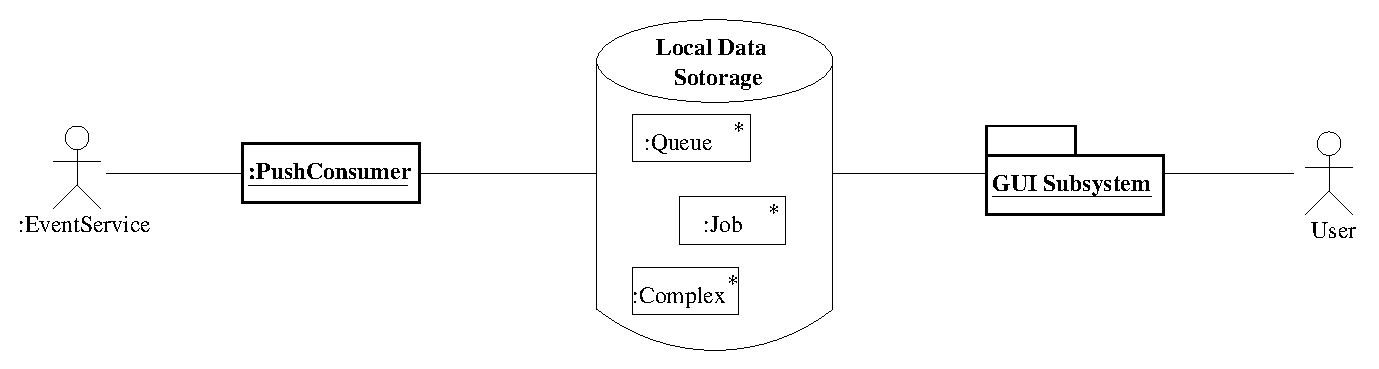
\includegraphics[width=\textwidth]{evclient.eps}
\caption{\label{f_user_ev_client}Typical logical structure of a \qidl\ event
client}
\end{figure}

\subsection{\label{s_user_using_qidl_rev}Using \qidl\ Revisited}
\subsubsection{Basic Events}
Programming with events is undoubtedly more work than programming a simple
\qidl\ client. But the gain in performance and application architecture is
worth the effort. As mentioned in the previous section, a \qidl\ event
consumer needs a local database representing the \codine\ objects, which is
updated upon the arrival of an event. It is beyond the scope of this example
to provide the complete code for this local storage or even the full client
program logic (display handling, user interaction, \dots). Furthermore will
the example only handle events for queues; other objects can be treated
similarly.

So let \texttt{MyQueue} be a C++ class that represents a \queue\ object in
the client, and \texttt{allQueues} be a global variable that stores all
queues in an STL vector class. The following example illustrates how to
register for events and handle them appropriately by updating the local data
storage. No synchronization with the actual client code---supposed to run in
a seperate thread---is done.
Let us take a look at the clients main program now. 

\begin{Verbatim}[frame=lines, numbers=left, fontsize=\small, framerule=1mm]
// forward decls
class MyQueue;
class EventClient;

// global data storage
vector<MyQueue*>   allQueues;

// the main program
int main(int argc, char** argv) {
   // initialize ORB, BOA, Context, QIDL Master, ...

   // setup event client
   EventClient* consumer = new EventClient(master);

   // start UI thread here
   // ...

   // accept events
   boa->impl_is_ready(...);

   return 0;
}
\end{Verbatim}

After the usual initialization tasks described in section 
\ref{s_user_using_common},
the main routine creates an object of type \texttt{EventClient} in line 13.
This is a custom class that does the actual event handling. After starting
one or more other threads to handle user input, the servant object is
connected to the CORBA bus by calling \texttt{impl\_is\_ready()} in line 19.
This blocks the main thread and incoming events are dispatched in the
\texttt{EventClient}'s \texttt{push()} function.

\begin{Verbatim}[frame=lines, numbers=left, fontsize=\small, framerule=1mm]
// class EventClient
class EventClient : virtual public CosEventComm_PushConsumer_skel {
   public:
      EventClient(Codine_Master_ptr master, CORBA_Context_ptr ctx);
      virtual ~EventClient {}

      virtual void push(const CORBA_Any& any);
      virtual void disconnect_push_consumer() {}
};

EventClient::EventClient(Codine_Master_ptr master,
                         CORBA_Context_ptr ctx) {
   // get consumer admin from master
   CosEventChannelAdmin_ConsumerAdmin_var     ca = 
                                 master->getConsumerAdmin(ctx);
   // get proxy push supplier from consumer admin
   CosEventChannelAdmin_ProxyPushSupplier_var pps = 
                                 ca->obtain_push_supplier();

   // connect as a push consumer
   pps->connect_push_consumer(
                  CosEventComm_PushConsumer::_duplicate(this));
}

void EventClient::push(const CORBA_Any& any) {
   // extract the event structure from the Any type
   Codine_event* ev;
   any >>= ev;

   // we're only interested in queues
   if(ev->obj != COD_QUEUE_LIST)
      return;

   // what type of event
   vector<MyQueue*>::iterator it;
   switch(ev->type) {
      case Codine_ev_add:
         // create a new queue representation from the supplied
         // contents and append it to the vector
         allQueues.push_back(new MyQueue(ev->changes));
         break;
      case Codine_ev_mod:
         // find the queue and update its state
         for(it=allQueues.begin(); it!=allQueues.end(); ++it)
            if((*it)->name() == ev->name)
               (*it)->update(ev->changes);
         break;
      case Codine_ev_del:
         // find the queue and remove it from the vector
         for(it=allQueues.begin(); it!=allQueues.end(); ++it)
            if((*it)->name() == ev->name) {
               delete *it;
               allQueues.erase(it);
            }
         break;
      default:
         break;
   }
}
\end{Verbatim}

The constructor (lines 11-23) retrieves the consumer administration interface
of the event channel from the \qidl\ master, where a proxy push supplier can
be obtained. It then connects to the channel as an event consumer in push
mode.

The \texttt{push()} method itself first extracts the \texttt{Codine::event}
structure from the delivered \texttt{Any} variable (lines 27-28). If the
concerned object is not a queue, then the event handler returns immediately,
since it is not interested in other objects (lines 30-32). The switch
statement in lines 36-58 distinguished the three event types: add, mod, and
del.

The \texttt{ev\_add} event is very easy to handle. Creating a new object from
the delivered \texttt{Codine::contentSeq} and appending it to the global data
storage is all there is to do (line 40). Both the \texttt{ev\_mod} and
\texttt{ev\_del} event handlers need to find the concerned object in the
local database (lines 44-45/50-51). If found, it is either updated with the
new object state (line 46), or deleted and removed from the global queue
vector (lines 52-53).

The actual work of maintaining the object state is of course delegated to the
\texttt{MyQueue} class. It must provide a consistent mapping of the delivered
\texttt{Codine::contentSeq} to its internal data representation---whatever
this might look like.

\subsubsection{The Event Counter}
Every \texttt{set\_} function returns an integer value. This return value is
a unique event count number that is sent with the event that was generated by
the \texttt{set\_} method. So if a client wants to be sure that it displays
the right object state at all times, especially after object modifications,
it should block and wait for the arrival of the corresponding event. The
pseudocode might look like this:

\begin{Verbatim}[fontsize=\small, frame=single]
void MyQueue::commitState() {
   count = queue_ref->set_state(myLocalState, ctx);
   blockOnConditionVariable(count);
}
\end{Verbatim}

After setting the queue's state, the local queue object blocks on a condition
variable which gets signaled when the event with number \texttt{count}
arrived. The signaling is done by the event handler, e.g. like in the
following pseudocode:

\begin{Verbatim}[fontsize=\small, frame=single]
void EventClient::push(CORBA_Any& any) {
   // ...
   switch(ev->type) {
      case Codine_ev_mod:
         // ...
         signalConditionVariable(count);
         break;
      // ...
   }
   // ...
}
\end{Verbatim}

If the incoming event modified an existing object, then the event handling
can simply signal the appropriate condition variable, thus waking up all
sleeping UI threads that were waiting for this event. These threads can then
safely update the display and be sure that the data shown is new enough to
reflect the changes made by the previous \texttt{commitState()} call.


\cleardoublepage
\section{\label{s_progdoc}\qidl\---The Implementor's View}
% supposed to be included by another LaTeX document
% as a section
This section describes \qidl\ from the developer's point of view. It explains
general concepts and ideas in section \ref{s_prog_overview}. Section
\ref{s_prog_idlgen} will focus in detail on one of the backbones of
\qidl---the \idlgen\ code generator. The inner workings of the server itself
will be described in section \ref{s_prog_server}.

\qidl\ was designed with some design patterns in mind. Their application is
outlined in section \ref{s_prog_patterns}. These and the overall structure of
\qidl\ make it easy to add new or extend existing functionality. Section
\ref{s_prog_extending} shows the right places to do so.

\subsection{\label{s_prog_overview}General Overview}
The \qidl\ CORBA server runs as as separate thread in the \codine\ master 
executable.
This thread sets up the \master\ object and then blocks and handles
incoming method invocations, while the other thread proceeds as if it ran as
a non-\qidl\ master, i.e. it waits for incoming \codapi\ requests, load reports,
etc. The code that actually executes \codapi\ and \qidl\ requests is exactly the
same. To be precise, each \qidl\ request invokes a local in-process 
\codapi\ request, i.e. one that is not sent over the network.

\subsubsection{Experiences and Concepts}
Several prototypes for evaluating the feasibility of the \qidl\ ideas were
developed and brought up the following results:

\paragraph{Creation of IDL, Header, and Core Implementation Files from Cull
           List Definitions}
  In order to ensure proper maintainability between the main \codine\
  source tree and the \qidl\ sources, the IDL files as well as some C++
  header and implementation files are automatically
  generated from the C header files defining the underlying cull lists. The
  existing cull list definition macros therefore had to be extended to
  provide sufficient information for automatic code generation.
  In addition to the IDL files, cull list definition headers in the standard
  macro format (without the extensions) can be generated. This is useful to
  produce headers for product distribution for use of standard {\tt cod\_api}
  by customers. Lex and yacc are used to scan and parse the C header files.

\paragraph{\qidl\ Integrated in \texttt{cod\_qmaster}}
  Using a separate server daemon for \qidl---as was planned for the first
  approach---requires duplication of all \codine\
  data structures (i.e. cull lists) and thus poses potential problems 
  concerning data integrity. It is therefore wiser to integrate \qidl\ into
  the \texttt{qmaster} executable as a separate thread.
  This offers even faster write access for CORBA clients,
  since their manipulations are directly made upon the master's data.

  The major drawback of this approach is that all read requests cause an
  increase of load in the master executable, thus slowing down performance.
  Even on multiprocessor machines potentially benefiting from
  multithreading, this may affect response times for execution daemons and
  the scheduler.
  In order to limit read access to the master's data,
  an easy-to-use CORBA event interface,
  multiplexed by a standard CORBA event service can propagate data
  changes to event listeners, as described in sections \ref{s_user_events}
  and \ref{s_user_using_qidl_rev}.

\paragraph{Security Problem}
  A standard CORBA compliant ORB offers no way of finding out which user
  sent a request or which host it came from.
  Commercial ORBs usually offer (proprietary) solutions to overcome this 
  problem, but these are usually not available on all desired platforms 
  (especially for LINUX). Furthermore are two different security
  implementations not interoperable, thereby forcing clients to be programmed
  with the same ORB product as the \qidl\ master.

  A glimpse of hope might come from the CORBA security service which is a
  standard CORBA common object service, but as its implementation requires
  modifications in the ORB itself, it is not likely that although two ORBs
  offer this service they will be able to exchange security data. Further
  evaluation will be necessary in this field. The proprietary authentication
  procedure presented in section \ref{s_user_authentication} provides a
  feasible means of passing the desired user and host information to the
  master, but is of course far from what deserves to be called \emph{secure}.

\paragraph{Objects and Lifetime}
  Upon startup, the \qidl\ server will
  create the singleton \master\ object that will always reside on the same
  TCP port (configured by environment variables, command line parameters
  or the like). This is necessary to produce the same IOR each time the 
  server starts.

  In addition to the {\tt Codine::Master} object, the server creates CORBA
  objects that represent the corresponding cull lists from qmaster. That is, all
  objects reside exactly once on one machine in one shared address space. 
  CORBA object references are by definition considered
  persistent. Nonetheless must a client be at any time aware of an object
  reference becoming invalid. This can have either physical reasons (broken
  network connection), logical reasons (a job may have terminated), or
  other reasons (server breakdown). In most of these cases some or all
  object references that a client holds will become invalid. The only
  exception to
  this rule is the {\tt Codine::Master} object, which is always reachable
  under the same address (as long as the server is running, of course).

\subsubsection{Multithreading}
The \qidl\ server consists of two threads: one for the more or less unchanged
\texttt{cod\_qmaster} code for the overall functionality and handling \codapi\
requests (from now on referred to as \emph{master thread}), and one for 
handling \qidl\ CORBA requests (to be called \emph{corba thread}). \qidl\ 
makes use of standard POSIX threads (\textsl{pthreads}) for portability reasons.

Both threads will spend most of the time blocking in a 
\texttt{select()} system call; the master thread waiting for data on the
\texttt{commd} port, the corba thread for requests on the BOA port.
These tasks, as well as marshaling and unmarshaling data, can be done
concurrently. The actual execution of the incoming requests is then mostly
done in the \codine\ kernel code, which is---for historical reasons---not
threadsafe. It is therefore necessary to disallow concurrent execution in the
\codine\ core, which is accomplished by obtaining (and releasing, of course) 
a global mutex variable, \texttt{master\_lock}. The general scheme of
execution is shown in figure \ref{f_prog_locking}, where the two lines
represent the master and corba threads, sequentializing when entering the
\codine\ kernel code.

\begin{figure}
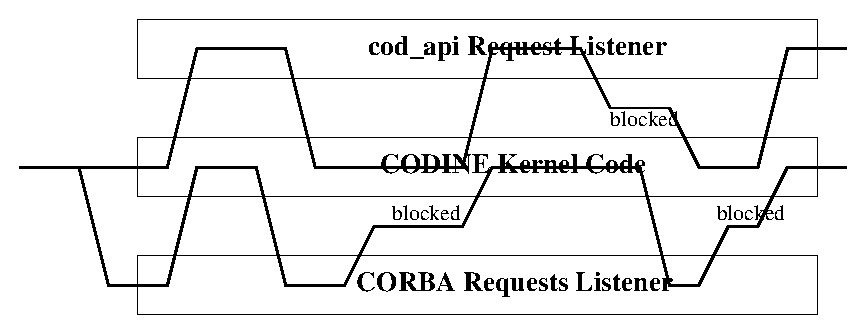
\includegraphics[width=\textwidth]{serverflow.eps}
\caption{\label{f_prog_locking}Concurrent and sequentialized execution of the
master and corba thread.}
\end{figure}

\paragraph{PthreadLock}
To simplify obtaining and releasing locks, a helper class was introduced for
\qidl. In fact, using an automatic class variable provides an elegant means to
release acquired locks in case of an unexpected exception. Consider the
following portion of code, using the standard POSIX C interface for threads:

\begin{Verbatim}[fontsize=\small, frame=single]
void send_event() {
   pthread_mutex_lock(&master_lock);
   
   // invoke CORBA request
   event_channel->push(last_event);
   
   pthread_mutex_unlock(&master_lock);
}
\end{Verbatim}

This code usually works fine. But invoking a CORBA request can always yield
an exception; be it a NIL object reference, a communication failure, or
whatever. In
this case, the \texttt{pthread\_mutex\_unlock()} command is never executed
and the lock never released. Instead of enclosing the critical sections in
explicit \texttt{try\dots catch} statements, a simple local variable solves
this problem in a more elegant way:

\begin{Verbatim}[fontsize=\small, frame=single]
void send_event() {
   PthreadLock lock(&master_lock); // this locks the mutex in the c'tor
   
   // invoke CORBA request
   event_channel->push(last_event);

   // leaving the block unlocks the mutex in the variable's d'tor
}
\end{Verbatim}

The local variable \texttt{lock} obtains the mutex variable when it is
created. Since C++ guarantees that all local objects' destructors are called
when they get out of scope, the lock is released no matter how the function
terminates.

Another advantage of using a class shows up when one function in a thread
(which has successfully acquired the lock) makes a call to another function,
which in turn tries to obtain the lock again. According to the pthreads
standard, this results in undefined behavior---usually a dead-lock. To solve
this problem, the \texttt{PthreadLock} class maintains an internal per-thread
reference count of each mutex variable. If one thread tries to acquire a lock
of a mutex variable more than once, it is not actually locked, but its
reference counter is increased---and decreased in the destructor, respectively.
If the reference count reaches zero, the mutex variable is actually
unlocked. \texttt{PthreadLock}'s interface is as follows:

\begin{Verbatim}[fontsize=\small, frame=single]
class PthreadLock {
   public:
      PthreadLock(pthread_mutex_t* m);
      ~PthreadLock();

      // avoid calling these unless you know what you're doing
      void     lock();
      void     unlock();
      
      static bool initialize();
   
   private:
      static bool init;

      static pthread_mutex_t lock;

      // stores a map<pthread_mutex_t*, unsigned int>
      static pthread_key_t key; 
      // the PthreadLock object's mutex
      pthread_mutex_t*     mutex;
      
      static void destroy(void* state)
         {delete (map<pthread_mutex_t*, unsigned int>*)state;}
};
\end{Verbatim}

\texttt{PthreadLock::initialize()} must be called before the first usage of
the class. It creates the pthread key variable, using the static
\texttt{PthreadLock::\-destroy()} function to cleanup memory. The per-thread
reference count is stored in a \texttt{map<pthread\_mutex\_t*, unsigned int>},
which associates the reference counter with its mutex. To further simplify
usage, the following macro is defined:

\begin{Verbatim}[fontsize=\small, frame=single]
#define AUTO_LOCK_MASTER PthreadLock lock(&master_lock);
\end{Verbatim}

\subsubsection{Source Files and their Dependencies}
The \qidl\ source directory is relatively small, whereas the ready compiled
executable can be several megabytes in size. That's because a large part of
the \qidl\ server code is automatically generated out of the api header
files. This makes the overall compilation process pretty complicated---and
thus the makefile, too.

\qidl\ is built around \emph{objects}, and that's why the makefile defines a
variable \texttt{OBJECTS} as:
\begin{Verbatim}[fontsize=\small, frame=single]
OBJECTS    = Queue. \
             ComplexEntry. \
             Complex. \
             Job. \
             PathName. \
             MailRecipient. \
             Variable. \
             ConfigEntry. \
             Configuration. \
             Range. \
             Calendar. \
             String. \
             Checkpoint. \
             QSCommand. \
             QueueingSystem. \
             ExecHost. \
             HostLoad. \
             LoadScaling. \
             PathAlias. \
             ParallelEnvironment. \
             Request. \
             SchedConf. \
             SubordinateQueue. \
             Usage. \
             UserEntry. \
             UserProject. \
             UserSet.
\end{Verbatim}
This contains the names of all interfaces and structs and can easily be
extended. A shell script called \texttt{make\_obj\_rules.sh}, which is
invoked by \texttt{make depend}, creates appropriate rules for these objects
to create their IDL, header, and implementation files. The overall dependencies
can be seen from figure \ref{f_prog_dependencies}.

\begin{figure}[b!]
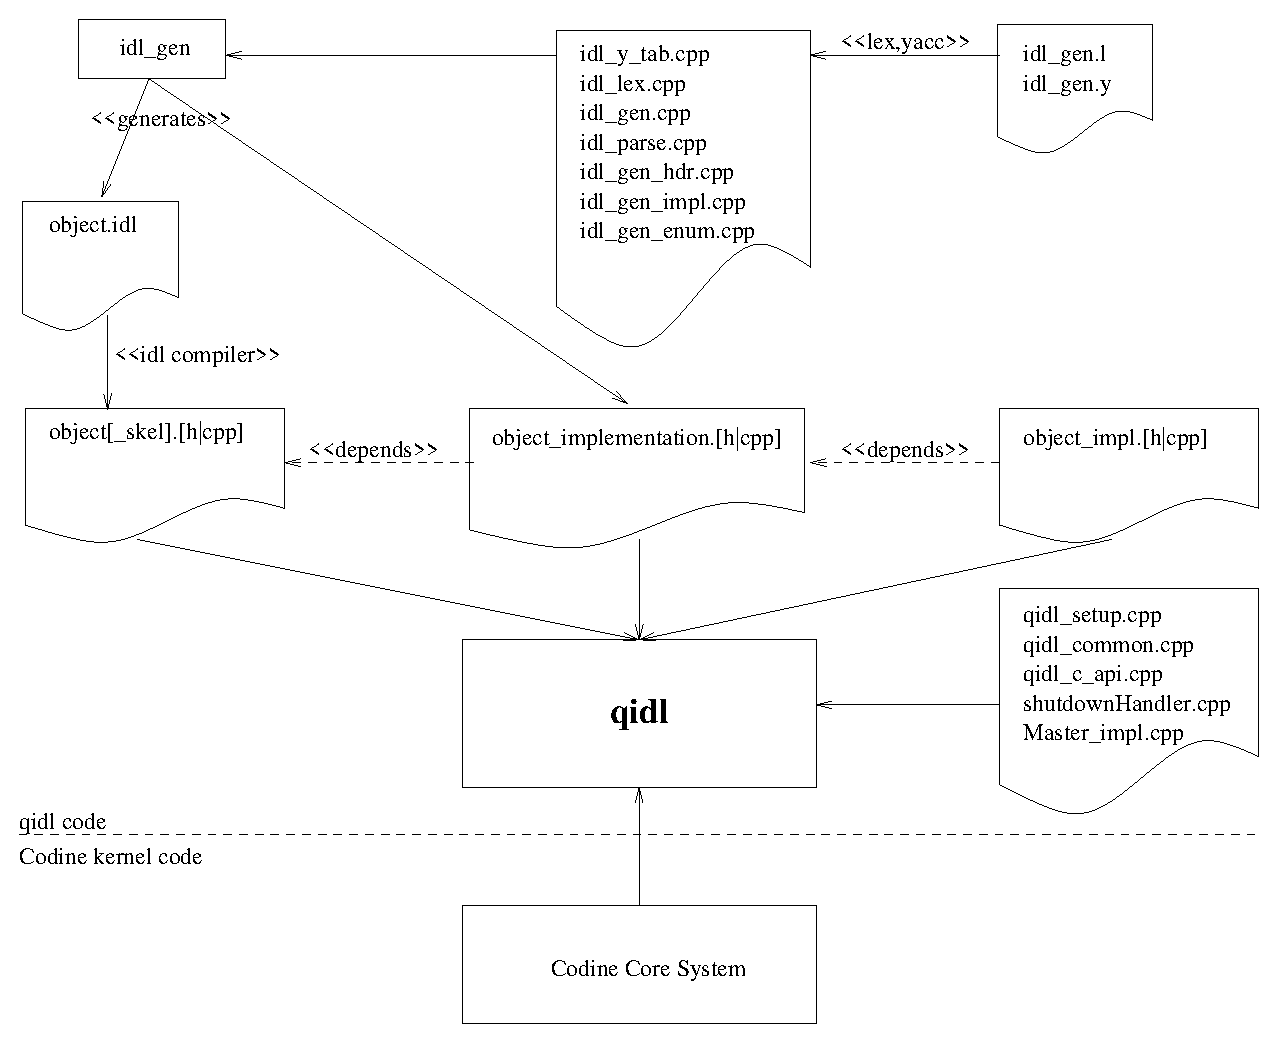
\includegraphics[width=\textwidth]{filedep.eps}
\caption{\label{f_prog_dependencies}The dependencies of the \qidl\ files.}
\end{figure}

Although some auxiliary files and header file dependencies have been
omitted, the diagram looks pretty complex, especially considering the
dependencies between \texttt{object\_skel, \_implementation,} and
\texttt{\_impl}, where the order of compilation and generation is extremely
important.

\subsection{\label{s_prog_idlgen}The Code Generator}
{\tt idl\_gen} is the utility to translate the cull list definitions from the
header files into 
\begin{itemize}
\item OMG CORBA IDL files
\item class headers for object implementation
\item partial object implementation
\item a file containing constants for attribute names.
\end{itemize}
It is also used to create headers for the
distribution release of {\tt cod\_api} cull headers. These headers will only
contain the standard cull list macros without any of the extensions
introduced in the following section. 

The command line syntax is as follows:

\begin{Verbatim}[fontsize=\small, frame=single]
idl_gen [-noidl] [-nohdr] [-noimpl] [-noelemcodes] [-nodisthdr] 
        input-files
        [-of files] [-oo objects]
\end{Verbatim}

where:
\begin{description}
\item[-noidl]      suppresses output of IDL files.
\item[-nohdr]      suppresses output of \texttt{\_implementation.h} files.
\item[-noimpl]     suppresses output of \texttt{\_implementation.cpp} files.
\item[-noelemcodes]suppresses output of \texttt{elem\_codes.idl} file.
\item[-nodisthdr]  suppresses output of .h.dist files.
\item[-of]         produces output only for objects that are defined in the
             following list of files.
\item[-oo]         produces output only for the given objects.
\item[input-files] is a list of files that contain cull list definitions.
\item[files]       is a list of files for whose objects output will be produced.
\item[objects]     is a list of object names for which output will be produced.
\end{description}

If -of or -oo are not given, \texttt{idl\_gen} produces output for all 
files or objects.  If specified, \emph{both} -oo and -of requirements must 
be met for an object.  That is, no output will be produced for the 
following command line:

\begin{Verbatim}[fontsize=\small, frame=single]
idl_gen cod_calendarL.h cod_queue.h -of cod_calendar.h -oo Queue
\end{Verbatim}

The order of the -oo and -of switches is not important as long as they occur 
after the input file list. It is also valid to have multiple -of and -oo
switches in one command line and to specify the same file or object more than 
once, or even to specify files that don't exist.
-of and -oo have no effect on distribution header output: .h.dist files are 
always produced, unless -nodisthdr is specified.

\texttt{idl\_gen} will create several files as shown in figure
\ref{f_prog_dependencies} on page \pageref{f_prog_dependencies}.
Since cull lists usually reference each other, the created files
will correctly \texttt{\#include} each other as appropriate. The program aborts
with an error when a reference could not be resolved successfully.

\subsubsection{Cull Macro Extensions}
As mentioned previously, the IDL and partial object implementation
files will be automatically 
generated from the C header files defining the cull lists. \idlgen\ 
(generated with the aid of lex and yacc) parses the desired header files 
and produces proper output files which do not have to be modified anymore and 
can thus be integrated smoothly in the build process via makefiles.

It is obvious that the previously existing macros for cull definition are by
far not sufficient for this purpose. The following paragraphs describe the 
extensions that have been necessary to accomplish this task.

It should be noted that these extensions are only required for the build
process of \qidl. In order to avoid unnecessary complexity of the header
files in the distribution and possible confusion of customers, it is highly
recommended that these extension only be used in the development tree of
\codine. \texttt{idl\_gen} offers a way to
produce standard cull list definition files out of the extended files.

\paragraph{List Definition}
\subparagraph{MACRO TYPE}
\begin{verbatim}
   LISTDEF
\end{verbatim}

\subparagraph{SYNTAX}
\begin{verbatim}
   ILISTDEF( type, name )
   SLISTDEF( type, name )
   XLISTDEF( type , name )
   LISTDEF( type )
\end{verbatim}

\subparagraph*{DESCRIPTION}
   This macro begins a list definition. The I and S forms will produce
   IDL output, where the name of the IDL interface is {\it name}. {\it Type}
   specifies the cull list type (e.g. JB\_Type). It is used by \qidl\
   for referencing objects.
      
   The ILISTDEF variant will produce a CORBA interface, whereas 
   SLISTDEF will create a struct. Use ILISTs for global
   objects and SLISTs for others. SLISTs need an additional parameter that
   specifies the name of the master list, where the objects are stored, e.g.
   MASTER\_QUEUE\_LIST for queues.
   
   The third form will not produce IDL output and should be used
   to indicate that no IDL interface will be generated.
   
   The last form is the standard list definition used by \codine. It will
   not produce IDL output and is considered obsolete but still supported
   for backward compatibility.

\paragraph{Standard List Entry}
\subparagraph{MACRO TYPE}
\begin{verbatim}
   COD_ELEM
\end{verbatim}

\subparagraph{SYNTAX}
\begin{verbatim}
   COD_ELEM( name )
   COD_RELEM( name )
   COD_IELEM( name )
   COD_IRELEM( name )
   COD_XELEM( name )
\end{verbatim}
   
   where ELEM is one of [ INT $|$ STRING $|$ FLOAT $|$ DOUBLE $|$ CHAR 
   $|$ LONG $|$ ULONG ]

\subparagraph{DESCRIPTION}
   These macros are used to define a list element for a cull list and/or a
   data member for an IDL interface/struct. The R variants produce a
   readonly attribute in IDL interfaces. In IDL structs and cull lists this
   shows no effect. Note that elements are not mapped to IDL attributes
   because of the context and raises clauses, but to get\_ and set\_ functions.

   The I variants produce data members only in IDL interfaces/structs but
   do not appear in cull lists. XELEMs are their counterpart: no IDL
   output, but standard cull meaning.

\paragraph{Object References And Aggregation}
\subparagraph{MACRO TYPE}
\begin{verbatim}
   COD_LIST, COD_OBJECT
\end{verbatim}

\subparagraph{SYNTAX}
\begin{verbatim}
   COD_TLIST( name, type )
   COD_ILIST( name, type )
   COD_RLIST( name, type )
   COD_IRLIST( name, type )
   COD_XLIST( name , type )
   COD_OBJECT( name, type )
   COD_IOBJECT( name, type )
   COD_ROBJECT( name, type )
   COD_IROBJECT( name, type )
   COD_XOBJECT( name, type )
   COD_LIST( name )
\end{verbatim}

\subparagraph{DESCRIPTION}
   These macros are used to define references to objects and aggregation of
   structs. All of them except ILIST and IOBJECT will result in a standard
   cull list entry as expected for LIST. The I variants will produce IDL output
   only. {\it name} is the name of the element that will appear in the cull list
   and in the IDL interface/struct (without prefix for the latter), and
   {\it type} is the type of interface/struct referenced and must be a type 
   that is defined with a LISTDEF macro. If the given type is unknown, no IDL 
   output will be generated for this entry.

   TLIST, ILIST, RLIST, and IRLIST  are used for sequences of the given type,
   whereas OBJECT references/contains exactly one instance of the given type.
   The R variants will produce a readonly attribute in objects and has no
   special meaning for IDL structs or cull lists.

   XLIST will not produce IDL output, but does appear in cull lists. The
   plain LIST variant without a type argument should be considered obsolete
   and is supposed to be replaced by XLISTs. This also serves documentation
   purposes.

   LIST is the old LIST macro with one parameter as
   used for cull lists before \qidl. It is considered obsolete and should
   not be used anymore. No IDL code is generated for this.

   TLIST should have actually be named LIST, but due to backwards
   compatibility to the old LIST macro another name had to be chosen.

\paragraph{Miscellaneous}
\subparagraph{MACRO TYPE}
\begin{verbatim}
   LISTEND
\end{verbatim}

\subparagraph{SYNTAX}
\begin{verbatim}
   LISTEND
\end{verbatim}

\subparagraph{DESCRIPTION}
   This macro ends a list definition and is not altered from the standard
   cull format.


\subparagraph{MACRO TYPE}
\begin{verbatim}
   IDL
\end{verbatim}

\subparagraph{SYNTAX}
\begin{verbatim}
   /*IDL
      idl_code
   XIDL*/
\end{verbatim}

\subparagraph{DESCRIPTION}
   Anything placed between and IDL/XIDL pair will be copied as is into the
   resulting IDL file. Use these "macros" to add special methods to an IDL
   interface.

   Note that the IDL section is a standard C multiline comment and will
   thus be ignored for cull lists. Be sure not to have other /* */ pairs
   between IDL and XIDL that may confuse the compiler. Only use // for
   IDL comments.

%\paragraph{Example}
%\begin{verbatim}
%CLISTDEF( JB_Type, Job )
%   COD_RULONG( JB_job_number )
%   COD_STRING( JB_script_file )
%   COD_XULONG( JB_uid )
%   COD_LIST( JB_stdout_path_list, PN_Type )
%   COD_IROBJECT( JB_queue, QU_Type )
%   COD_XLIST( JB_hard_queue_list, QR_Type )
%   COD_ILIST( JB_hard_queue_list, QU_Type )
%   IDL
%      void suspend();  // suspends this job
%   XIDL
%LISTEND
%
%SLISTDEF( PN_Type, PathName )
%   STRING( PN_path )
%   STRING( PN_host )
%LISTEND
%\end{verbatim}
%
%This excerpt from a C header file produces the following IDL code:
%
%\begin{verbatim}
%module Codine {
%   interface Job : Obj {
%      readonly attribute ulong job_number;
%               attribute string script_file;
%               attribute PathNameSeq stdout_path_list;
%      readonly attribute Queue queue;
%               attribute QueueSeq hard_queue_list;
%      void suspend();  // suspends this job
%   };
%
%   struct PathName {
%      string path;
%      string host;
%   };
%};
%\end{verbatim}

\subsubsection{Lex and Yacc}
\texttt{lex} and \texttt{yacc} will be used to produce a parser for cull
header files. This parser understands the keywords defined in the previous
section, "Cull Macro Extensions", and ignores everything else. The main
program (\texttt{idl\_gen.cpp}) will call this parser on all input files,
thus generating meta information stored in the data structures defined in
\texttt{idl\_repository.h}. It then calls several functions
that analyze the meta data and generate the desired
output. The distribution headers (if desired) are generated on the fly when
parsing the input files.

In the parsing process itself, the meta data structures are filled. These are
simple structs containing information for each parsed cull list and its
elements. This includes mainly names and data type information. They make
extensive use of the C++ Standard Template Library (STL) and can be accessed
easily. The actual code generator functions iterate over the meta data and
produce the desired output.

\subsubsection[From Cull to IDL]{\label{s_prog_skeleton}
                             From Cull to IDL---Or: The Server Skeleton}
The most important files generated by \idlgen\ are the OMG CORBA IDL files,
describing the public interfaces of the \codine\ objects. All interfaces are
embedded in a namespace \texttt{Codine} and derived from the base interface
\texttt{Codine::Obj}. There is not very much to do for the IDL code
generator. Apart from writing the file header and footer, it creates a
\texttt{get\_} and (if not read-only) a \texttt{set\_} function for each
element in the list's meta data structure, always appending the
\texttt{raises} and \texttt{context} clauses. The last task is to append the
inlined \texttt{/*IDL\dots XIDL*/} code from the cull list definitions.

\subsubsection[Basic Implementation]{\label{s_prog_flesh}
                     Basic Implementation---Or: The Flesh around the Bones}
Creating the implementation header and source files is by far more complicated
than creating the IDL files. That is to say that the \emph{creation}
itself is not difficult---it only consists of some stream operations just like 
the ones for the IDL files. The intelligence lies in the \emph{contents} of
the produced files, which provide code that otherwise would have to be written 
by hand in an ever-reoccuring pattern. Now let's take a look at the details of 
the files.

\paragraph{Implementation Header}
The \texttt{\_implementation.h} file contains a complete class declaration
for an IDL interface implementation (conforming to ORBacus' BOA
implementation). It is therefore derived \texttt{public virtual} from the
corresponding \texttt{\_skel} class created by the IDL compiler from the IDL
file. Apart from constructor and destructor, the class declares prototypes of
all methods defined in the object's interface. Functions that involve
references to other objects (not structs!) are declared pure virtual, i.e.
they have to be implemented by yet another subclass, as described in section
\ref{s_prog_server_objects}.

There are some other class members as well. To be precise, these are:
\begin{Verbatim}[fontsize=\small, frame=single]
class Some_implementation : virtual public Some_skel {
   // ...

   protected:
      CORBA_String_var          key;
      lListElem*                self;
      lListElem*                newSelf;
      virtual lListElem*        getSelf() = 0;
      CORBA_ORB_var             orb;
      time_t                    creation;
      cod_ulong                 lastEvent;
   friend class Codine_Master_impl;
};
\end{Verbatim}
\begin{description}
\item[key] is the unique object name. For jobs this is not a string but an
integer value.
\item[self] is a pointer to the object's underlying cull list.
\item[newself] is used in conjunction with events.
\item[getSelf()] returns a pointer to the object's underlying cull list. This
function must be implemented by a subclass and usually makes an 
\texttt{lFindFirst()} call.
\item[orb] is the ORB's object reference.
\item[creation] is the object's creation time. It is non-zero for newly
created objects (i.e. those visible only to their creator).
\item[lastEvent] is the integer value of the last event associated with this
object.
\end{description}

\paragraph{Implementation File}
The \texttt{\_implementation.cpp} file is more interesting. It mainly
contains the implementations of all \texttt{get\_} and \texttt{set\_}
functions except the ones that concern references to other \codine\ objects.
The first lines of each of these functions are exactly identical and look
like this (taken from \texttt{Codine\_Queue\_implementation::\-get\_qhostname}):

\begin{Verbatim}[fontsize=\small, frame=single]
cod_string Codine_Queue_implementation::get_qhostname(
                                          CORBA_Context* ctx) {
   QENTER("Queue::get_qhostname");
   AUTO_LOCK_MASTER;
   qidl_authenticate(ctx);
   if(!getSelf()) {
      orb->disconnect(this);
      CORBA_release(this);
      throw Codine_ObjDestroyed();
   }

   // ...
}
\end{Verbatim}

These commands
\begin{enumerate}
\item print debug/trace output,
\item acquire the global mutex variable,
\item validate the delivered context variable (throws an exception in case
      of an error),
\item retrieve the object's underlying cull list, and if this is not
      successful
   \begin{enumerate}
   \item disconnects the CORBA object from the ORB, and
   \item throws an appropriate exception.
   \end{enumerate}
\end{enumerate}

This block is followed by some attribute and data type specific lines, like
these for a string type:

\begin{Verbatim}[fontsize=\small, frame=single]
cod_string Codine_Queue_implementation::get_qhostname(
                                       CORBA_Context* ctx) {
   // ...

   char* temp = lGetString(self, QU_qhostname);
   cod_string foo = CORBA_string_dup(temp?temp:"");
   return foo;
}
\end{Verbatim}

Comparing this to a \texttt{cod\_ulong} typed attribute reveals a common
pattern:

\begin{Verbatim}[fontsize=\small, frame=single]
cod_ulong Codine_Queue_implementation::get_seq_no(CORBA_Context* ctx) {
   // ...

   cod_ulong foo = lGetUlong(self, QU_seq_no);
   return foo;
}
\end{Verbatim}

\begin{enumerate}
\item Retrieve the attribute's value from the cull,
\item make a copy of the value considering a NULL pointer (strings only), and
\item return the value.
\end{enumerate}

Very easy, isn't it? If this code wasn't generated automatically, someone
would have to hand-write code like this for hundreds of attributes---cearly
unsatisfying. What about attributes with structs as their data type? Here's
the code:

\begin{Verbatim}[fontsize=\small, frame=single]
Codine_ComplexEntrySeq* 
      Codine_Queue_implementation::get_consumable_config_list(
      CORBA_Context* ctx) {
   // ...

   lList* lp = lGetList(self, QU_consumable_config_list);
   Codine_ComplexEntrySeq* foo = cull2ComplexEntrySeq(lp);
   return foo;
}
\end{Verbatim}

\label{p_converters}
The only difference is the call to the \texttt{cull2ComplexEntrySeq()}
function. As its name implies, it converts a cull list to a
\texttt{Codine::ComplexEntrySeq}. There are many functions like
\texttt{cull2XXXSeq()} and \texttt{XXXSeq2cull()} which convert CORBA
sequence types to and from their corresponding cull list type. In spite of
all automation, these functions have to be written by hand, but they are
really easy and need not be mentioned here.

The \texttt{set\_} functions are somewhat more interesting. Each of these
requests is translated into a local \codapi\ request because
\begin{itemize}
\item \codapi\ is a tested and reliable interface,
\item it eliminates the danger of data inconsistency, since data is manipulated
      by the same portion of code for both \codapi\ and \qidl\ requests,
\item user access rights need not be checked explicitly for a \qidl\ request,
\item proper event handling is guaranteed for both \qidl\ event clients and 
      the \codine\ scheduler.
\end{itemize}
So the code looks as follows:

\begin{Verbatim}[fontsize=\small, frame=single]
cod_ulong Codine_Queue_implementation::set_qhostname(const char* val,
                                                  CORBA_Context* ctx) {
   // usual function header omitted...

   if(creation != 0) {
      lSetString(self, QU_qhostname, (char*)val);
      return 0;
   }

   lListPtr      lp;
   lListPtr     alp;
   lListElem*   lep;
   lEnumeration* what;

   lp = lCreateList("My qhostname list", QU_Type);
   lAppendElem(lp, (lep = lCopyElem(self)));
   lSetString(lep, QU_qhostname, (char*)val);
   what = lWhat("%T(%I %I)", QU_Type, QU_qname, QU_qhostname);
   alp = cod_api(COD_QUEUE_LIST, COD_API_MOD, &lp, NULL, what);
   lFreeWhat(what);
   throwErrors(alp);
   return lastEvent;
}
\end{Verbatim}

The function first checks if the object's creation time is non-zero, i.e. if
the object is still "under construction" by a user and not yet publicly
visible. In this case, the modification of the attribute can be done in the
local \texttt{self} cull list. Since no event will be generated for this,
the function returns 0 as the event number.

The other case, i.e. modifying a global object requires a bit more work.
\codapi\ programmers might find the code familiar. All there is to do is
\begin{enumerate}
\item setting up a cull list,
\item appending a copy of the object's cull,
\item modifying the appropriate value,
\item setting up an \texttt{lEnumeration} to define the scope of the request,
\item issue the \codapi\ call, 
\item cleaning up the data structures, and
\item returning the event number to the caller.
\end{enumerate}

There are two features worth mentioning here. The first one is the \codapi\
call itself. It looks like a standard \codapi\ invocation, one like any other
\codapi\ could have done, too. The only difference is that the function's
implementation recognizes that it was called from \emph{inside} the master
executable and thus does not send the request over the network, but simply
passes it on directly to the receiver function.

The second feature concerns the 6th item, cleaning up. The attentive reader
may have noticed that the cull lists are not freed with a call to
\texttt{lFreeList()}. That is because the standard \texttt{lList*}s have been
replaced by a \texttt{lListPtr} class, which cares for automatic memory
management and defines some conversion functions for convenient usage in the
standard \codapi\ context.

Like the \texttt{PthreadLock} facility, this feature was driven by 
Elegan$C^{++}$e concerning exception handling. Notice the line
\texttt{throwErrors(alp);} in the code above. This is a custom function that
converts the answer list returned by a \codapi\ call into a
\texttt{Codine::Error} exception---if an error occured, that is. If
everything went well, nothing happens and the function returns happily. In
both cases, the lists' memory has to be freed, which would require ugly
\texttt{try\dots catch} clauses, hadn't these \texttt{lListPtr} classes been
used.

The code for setting attributes with fundamental data types other than
string is very similar to the one shown above. Even handling \texttt{struct}
types isn't really more work:

\begin{Verbatim}[fontsize=\small, frame=single]
cod_ulong Codine_Queue_implementation::set_migr_load_thresholds(
               const Codine_ComplexEntrySeq& val, 
               CORBA_Context* ctx) {
   // ...

   lp = lCreateList("My migr_load_thresholds list", QU_Type);
   lAppendElem(lp, (lep = lCopyElem(self)));
   lSetList(lep, QU_migr_load_thresholds,
               ComplexEntrySeq2cull((Codine_ComplexEntrySeq&)val));
   what = lWhat("%T(%I %I)", QU_Type, QU_qname, QU_migr_load_thresholds);
   alp = cod_api(COD_QUEUE_LIST, COD_API_MOD, &lp, NULL, what);
   lFreeWhat(what);
   throwErrors(alp);
   return lastEvent;
}
\end{Verbatim}

The only real difference is the call to \texttt{ComplexEntrySeq2cull()},
which does exactly that. See page \pageref{p_converters} earlier in this
section for more information.

The last major content of the \texttt{\_implementation.cpp} file is the
implementation of get \texttt{get\_} and \texttt{set\_content()} functions.
These are usually lengthy methods, since they must assemble or disassemble a
\texttt{Codine::contentSeq} that represents the complete object state.
\texttt{get\_content()} is significantly easier to write than
\texttt{set\_content()}, because the latter requires some tricky, admittedly 
hard to understand code. But let's start with the first of the two,
\texttt{get\_content()}:

\begin{Verbatim}[fontsize=\small, frame=single]
Codine_contentSeq* Codine_Queue_implementation::get_content(
                                                CORBA_Context* ctx) {
   // usual function header ...

   // build content sequence
   Codine_contentSeq* cs = new Codine_contentSeq;
   char* dummy;

   cs->length(24);         // i.e. the number of attributes

   // qname
   cs->operator[](0).elem = Codine_QU_qname;
   cs->operator[](0).value <<= CORBA_string_dup(
                     (dummy = lGetString(self, QU_qname))?dummy:"");
   // seq_no
   cs->operator[](4).elem = Codine_QU_seq_no;
   cs->operator[](4).value <<= (cod_ulong)lGetUlong(self, QU_seq_no);
   // load_thresholds
   cs->operator[](5).elem = Codine_QU_load_thresholds;
   cs->operator[](5).value <<= get_load_thresholds(
                   Codine_Master_impl::instance()->getMasterContext());
   // complex_list
   cs->operator[](22).elem = Codine_QU_complex_list;
   cs->operator[](22).value <<= get_complex_list(
                   Codine_Master_impl::instance()->getMasterContext());
   // other attributes follow...
   
   return cs;
}
}\end{Verbatim}

This code is pretty straightforward. The function simply sets up a
\texttt{content\-Seq} and fills its entries with reasonable name/value
pairs. For \texttt{struct} and reference type attributes, it makes use of its
own \texttt{get\_} functions described earlier in this subsection. This is
possible, since the \texttt{value} of the \texttt{Codine::contentSeq} is of
type \texttt{CORBA::Any}, and with the \texttt{<<=} operator virtually any
user defined type can be assigned to the \texttt{value} variable.

For the \texttt{set\_content()} method, the code is not quite that simple:

\begin{Verbatim}[fontsize=\small, frame=single]
cod_ulong Codine_Queue_implementation::set_content(
               const Codine_contentSeq& cs, CORBA_Context* ctx) {
   // usual function header...

   // intermediate variables, not all may be used
   Codine_ComplexEntrySeq* ComplexEntry_val;
   Codine_ComplexSeq* Complex_val;
   cod_float Float_val;
   cod_double Double_val;
   cod_ulong Ulong_val;
   cod_long Long_val;
   cod_char Char_val;
   cod_int Int_val;
   cod_string String_val;
   lList* List_val;
   lListPtr lp = lCreateList("set content", QU_Type);
   lListElem* lep = lCreateElem(QU_Type);
   lAppendElem(lp, lep);

   // now pretend we're CORBA-only
   time_t old_creation = creation;
   creation = 1;
   lListElem* oldSelf = self;
   self = lep;
   
   // check the sequence
   for(CORBA_ULong i=0; i<cs.length(); i++) {
      switch(cs[i].elem) {
      case QU_qname:
         cs[i].value >>= String_val;
         lSetString(lep, QU_qname, String_val);
         break;
      case QU_seq_no:
         cs[i].value >>= Ulong_val;
         lSetUlong(lep, QU_seq_no, Ulong_val);
         break;
      case QU_load_thresholds:
         cs[i].value >>= ComplexEntry_val;
         List_val = ComplexEntrySeq2cull(*ComplexEntry_val);
         lSetList(lep, QU_load_thresholds, List_val);
         break;
      case QU_complex_list:
         cs[i].value >>= Complex_val;
         set_complex_list(*Complex_val, 
                  Codine_Master_impl::instance()->getMasterContext());
         break;
   }

   // don't forget to set back
   creation = old_creation;
   self = oldSelf;

   // now set the state
   if(creation) {
      lFreeElem(self);
      self = lCopyElem(lep);
   }
   else {
      lListPtr alp;
      lEnumeration* what = lWhat("%T(ALL)", QU_Type);
      alp = cod_api(COD_QUEUE_LIST, COD_API_MOD, &lp, NULL, what);
      lFreeWhat(what);
      throwErrors(alp);
   }

   return lastEvent;
}
}\end{Verbatim}

Have a look at the \texttt{for} loop in the middle of the code, first. It
iterates through the given sequence and checks which elements are supplied in
it. Note that this sequence need not be complete and can come in any order,
so the \texttt{for} and \texttt{switch} statements are necessary.
First of all, the content of the \texttt{Any} value has to be extracted into
local variables, declared at the top of the code. The \texttt{>>=} operator
ensures type safety here. 

For simple and \texttt{struct} types, simply setting the extracted value
(converting it to a cull list for \texttt{struct}s) in the soon-to-be new
object state cull is all there is to do. Object reference types (such as the
\texttt{complex\_list} above) make things more complicated. You can see, that
again, it's only one line of code, \texttt{set\_complex\_list(\dots)}. But to
make this work, several preconditions have to be met.

First of all, the object must pretend that it is \emph{CORBA-only}, i.e. not
publicly visible to all \codine\ users, since the latter would force the
\texttt{getSelf()} method, called by the \texttt{set\_complex\_list()} method
to get the current object state from the \codine\ master object store, thus
overriding any local changes made up to this point. Then it has to
temporarily set the \texttt{self} variable to the above mentioned soon-to-be
new object state cull. This makes \texttt{getSelf()} return this (actually
local) variable and \texttt{set\_complex\_list()} alter the correct value.
This mechanism would work for all attributes, too, and not only for object
reference types. But the simplicity of inline implementation and the
otherwise necessary function call overhead (including the usual function
header, remember) makes the current implementation much faster.

After the cull list has been set up correctly for all delivered attributes,
the changed variables \texttt{creation} and \texttt{self} are reset to their
original values. Then the new object state is either set locally, or set as
the global state with a \codapi\ call. This creates an event, and its counter
is returned from the function.

The \idlgen\ code generator provides a broad basis that the \qidl\ server can
be built upon. Especially the two \texttt{\_implementation.[h$|$cpp]} files
relief the programmer of some monotonous and error-prone copy\&paste work.
But still some parts have to be implemented by hand, as described in the
following section.

\subsection[The Server]{\label{s_prog_server}The Server---Or: Adding Skin 
                                             and Brain}
Think of the \qidl\ servers as a human (or, for that matter, any mammal)
body: There's a skeleton, forming the overall shape. This is
represented by the IDL interfaces, described in section
\ref{s_prog_skeleton}. The body's muscles and flesh strengthen its structure
and provide the means to accomplish some simple tasks---the server's base
implementation as presented in section \ref{s_prog_flesh}. To round off the
body's overall appearance and to bring life and meaning to it, it needs skin
(additional and convenience functions) and---most important---a brain, i.e.
the \master\ object. It's like having Frankenstein's monster assembled
automatically, just adding the interesting parts by hand. The following
subsections show how this is done for the \qidl\ "monster".

\subsubsection{The Master}
Recall from section \ref{s_userdoc} that the \master\ object is the entry point
for a \qidl\ client into the \codine\ system. From here, all other objects
can be accessed and new ones created. Event handling and other functions are
offered, too. Let's take a look at the master's header file. The remainder of
this subsection will pinpoint some important and interesting features of its
implementation and frequently refers to some lines is this header file. You
may want to skip back to this page and have a closer look at the referenced
class members. You may also find a comparison with the master's IDL file 
valuable in understanding the overall concept.

\begin{Verbatim}[frame=lines, numbers=left, fontsize=\small, framerule=1mm]
class Codine_Master_impl : virtual public OBEventHandler, 
                         virtual public Codine_Master_skel, 
                         virtual public CosEventComm_PushSupplier_skel {
   private:
      static Codine_Master_impl* master;

   protected:
      Codine_Master_impl(CORBA_ORB_ptr o, CORBA_BOA_ptr b);
      virtual ~Codine_Master_impl();

      // OBEventHandler stuff, sends event when notified
      virtual void handleEvent(OBMask mask);
      virtual void handleStop();

   public:
      // singleton retrieval
      static Codine_Master_impl* instance();
      const char*                getIOR();

      // idl methods
      virtual Codine_QueueSeq*         getQueues();
      virtual Codine_QueueSeq*         getQueues(CORBA_Context_ptr ctx);
      virtual Codine_JobSeq*           getJobs();
      virtual Codine_JobSeq*           getJobs(CORBA_Context_ptr ctx);
      virtual Codine_ComplexSeq*       getComplexes();
      virtual Codine_ComplexSeq*       getComplexes(CORBA_Context* ctx);
      // similar for all other objects


      virtual Codine_Queue*            newQueue(const char* name,
                                                CORBA_Context* ctx);
      virtual Codine_Complex*          newComplex(const char* name,
                                                  CORBA_Context* ctx);
      // similar for all other objects


      virtual CosEventChannelAdmin_ConsumerAdmin* getConsumerAdmin(
                    CORBA_Context* ctx);
      virtual CORBA_Boolean                       registerObject(
                    CORBA_ULong, class CORBA_Object *);
      virtual CORBA_Boolean                       unregisterObject(
                    CORBA_ULong, class CORBA_Object *);

      virtual void                      disconnect_push_supplier();

      virtual void shutdown(CORBA_Context* ctx);

      // static methods for creation and destruction
      static bool  initialize(CORBA_ORB_ptr o, CORBA_BOA_ptr b); 
      static void  exit();
      
      // handling events
      void         deleteObject(int type, const char* name);
      void         deleteObject(int type, cod_ulong id);
      void         addObject(int type, const char* name);
      void         addObject(int type, cod_ulong id);
      void         addEvent(const CORBA_Any& any);

      // finding objects
      list<Codine_Queue_impl*>::iterator         
                           getQueue(const char* name);
      list<Codine_Complex_impl*>::iterator
                           getComplex(const char* name);
      list<Codine_Job_impl*>::iterator          
                           getJob(cod_ulong name);
      // you get the point ...

      Codine_Queue_impl*            getQueueImpl(const char* name);
      Codine_Complex_impl*          getComplexImpl(const char* name);
      Codine_Job_impl*              getJobImpl(cod_ulong name);
      // and again ...

      // misc
      CORBA_Context*                getMasterContext();

   private:
      // all static since we are a singleton
      static CORBA_BOA_var                               boa;
      static CORBA_ORB_var                               orb;
      static list<Codine_Queue_impl*>                    queues;
      static list<Codine_Complex_impl*>                  complexes;
      static list<Codine_Job_impl*>                      jobs;
      static list<Codine_Configuration_impl*>            configurations;
      // similar for other objects...
      static queue<CORBA_Any>                            events;
      static pthread_mutex_t                             events_lock;
      static CosNaming_Name_var                          name;
      static CosNaming_NamingContext_var                 ns;
      static CosEventChannelAdmin_EventChannel_var       es;
      static CosEventChannelAdmin_ProxyPushConsumer_var  ev_consumer;
      static int                                         obEventFd[2];
      static CORBA_Context_var                           ctx;

   friend class ShutdownHandler;
};
\end{Verbatim}

This seems quite complicated, but fortunately it isn't really that difficult.
But always keep in mind that this class has two faces: The public IDL
interface implementation and the non-public interface to fulfill \qidl\
internal tasks. Not only has the class two faces, it also has three base
classes (lines 1-3): \texttt{OBEventHandler} (an internal one, more on that 
later), \texttt{Codine\_Master\_skel} (of course), and
\texttt{CosEventComm\_PushSupplier\_skel} (to send events). Luckily, there's
only one instance of the class allowed (a \emph{singleton}, see section
\ref{s_prog_singleton}). Its pointer is stored in the static \texttt{master}
variable (line 5).

\paragraph{Initialization and Setup}
Now that's enough numbers for the moment. Let's take a look at the master's
setup tasks. These are executed exactly once, since it is a singleton object.
It's one and only reference can be retrieved by the \texttt{instance()} method,
and is set up by \texttt{initialize()}. The constructor is protected to prevent
unwanted instantiation. It binds the object to the naming service, and tries
to connect to the event service for sending events. There is nothing special
to explain here; it's all standard CORBA code.

The static \texttt{initialize()} function creates a \master\ object and
creates a CORBA representation for all objects in the cluster. For complexes,
this looks like

\begin{Verbatim}[fontsize=\small, frame=single]
   complexes.clear();
   for_each_cpp(lep, Master_Complex_List) {
      Codine_Complex_impl* c = new Codine_Complex_impl(
                                    lGetString(lep, CX_name), orb);
      complexes.push_back(c);
      orb->connect(c);
   }
 \end{Verbatim}

\texttt{complexes} is one of the static data members of the
\texttt{Codine\_Master\_impl} class. They are declared in lines 80-84. There
is one list for each class of \codine\ objects. There is not really very much
to do apart from constructing the objects and appending them to the list.
Similar code is executed for all types of objects.

To destroy the singleton object, there is either the static \texttt{exit()}
function, which cares for deletion of all objects, or the \texttt{destroy()}
method as declared in the object's interface. This function checks for the
appropriate privileges of the caller and then calls \texttt{exit()} to shut
down properly.

\paragraph{Object Management}
Apart from implementing the \texttt{getXXXs()} methods declared in the
master's IDL interface---which is a pretty trivial task, simply converting
the STL lists to a CORBA sequence---the \qidl\ master must keep track of
objects being added or deleted when the server is running. It therefore
declares \texttt{addObject()} and \texttt{deleteObject} functions (lines
53-56), that manage the object lists and generate the appropriate events (see
the next paragraph on event handling). These functions are called from within
\codine\ kernel code that process \codapi\ requests (both internal and
external ones). 

For easy internal access to objects, there are functions like
\texttt{getQueue(name)}, or \texttt{getJob(id)} that return a list iterator
that points to the desired object (or \texttt{end()}, if it does not exist).
\texttt{getQueueImpl()} and \texttt{getJobImpl()} return the object itself.
Their implementation is straightforward and looks like this:

\begin{Verbatim}[fontsize=\small, frame=single]
// getQueues()
list<Codine_Queue_impl*>::iterator Codine_Master_impl::getQueue(
                                                const char* name) {         
   QENTER("Master::getQueue");

   list<Codine_Queue_impl*>::iterator  qelem;
   for(qelem=queues.begin(); qelem != queues.end(); ++qelem)
      if(!strcmp((*qelem)->key, name)) 
         return qelem;

   return qelem;
}

Codine_Queue_impl* Codine_Master_impl::getQueueImpl(const char* name) {
   QENTER("Master::getQueueImpl");

   list<Codine_Queue_impl*>::iterator  qelem = getQueue(name);
   if(qelem != queues.end())
      return *qelem;
   else
      return NULL;
}
\end{Verbatim}

\paragraph{Internal Event Handling}
The following pages will explain a pretty complicated feature: the
event handling facility. The difficulty is not to become confused with two
different event handling concepts: CORBA events and ORBacus events. The
former are sent across the network to event consumers via the CORBA event
channel. The latter are \emph{internal} events offered by ORB\-acus that allow
a program to "hook" itself into the ORBacus message queue and take over the
flow of control. It can do so by having a class derive from
\texttt{OBEventHandler} and implement the two functions from lines 12 and 13.

The basic principle is simple. Someone has to register an instance of a
\texttt{OBEventHandler}-derived class with the ORBacus ORB and specify a file
descriptor to connect with it. If a read or write event occurs for this file
descriptor, the object's \texttt{handleEvent()} method is called. This
mechanism is the only way for \qidl\ to send a message from the master thread
to the corba thread, especially when the latter is waiting for CORBA
requests. To demonstrate this, take a look at the \texttt{shutdownHandler}
class:

\begin{Verbatim}[fontsize=\small, frame=single]
class ShutdownHandler : public OBEventHandler {
   public:
      ShutdownHandler(); 
      virtual ~ShutdownHandler(); 

      virtual void handleEvent(OBMask mask); 
      virtual void handleStop();

   public:
      static int     fd[2];         // the fd I am listening to
};

// implementation 
int ShutdownHandler::fd[2] = {1,1};

ShutdownHandler::ShutdownHandler() {
   pipe(fd);
   OBReactor* Reactor = OBReactor::instance(); 
   Reactor -> registerHandler(this, OBEventRead, fd[0]);
}

ShutdownHandler::~ShutdownHandler() {
   close(fd[0]);
   close(fd[1]);
   OBReactor* Reactor = OBReactor::instance();
   Reactor -> unregisterHandler(this);
}

void ShutdownHandler::handleEvent(OBMask mask) {
   Codine_Master_impl::boa->deactivate_impl(NULL);
}
\end{Verbatim}

This class is used when a user issues a \texttt{qconf -km} command to
shutdown \codine. This request is handled in the master thread, but somehow
the corba thread must be signaled to shut down properly. This is down by
writing one byte (no matter what it contains) into the public pipe set up by
the object's constructor. This causes ORBacus to invoke the
\texttt{ShutdownHandler::handleEvent} method which simply signals the BOA to
disconnect from the CORBA bus. All objects are freed correctly, then.

A very similar, but a trifle more complicated mechanism is used when the
master thread needs to signal the corba thread to send a CORBA event. Figure
\ref{f_prog_event} shows the logical flow of control and data 
for this scenario.

\begin{figure}
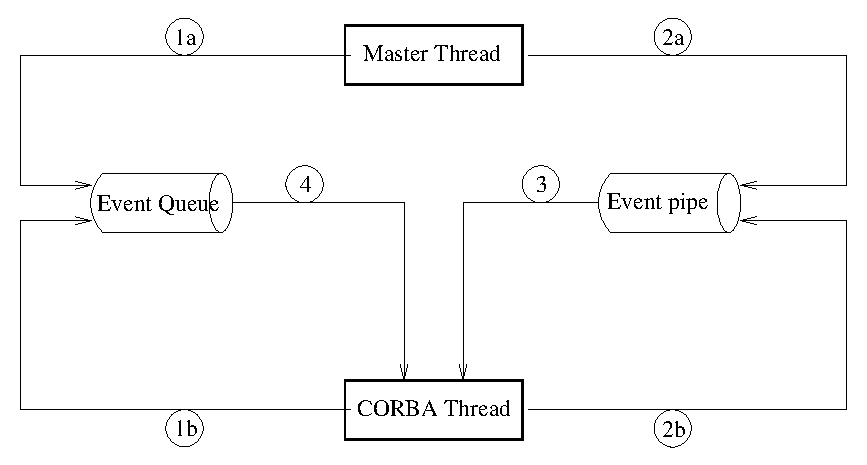
\includegraphics[width=\textwidth]{eventflow.eps}
\caption{\label{f_prog_event}Flow of control and data for event handling}
\end{figure}

\begin{enumerate}
\item The event itself is pushed into the master's event queue (defined in
line 85 in the \master\ header file). This can be done by either the
master thread (case a, responding to a \codapi\ request), or by the 
corba thread (case b, responding to a \qidl\ request).
This is the real \texttt{Codine::event} struct that is actually sent across
the network to the event channel.
Of course, the appropriate locks for the event queue must be obtained 
and released correctly.
\item A byte is written into the ORBacus event handler's pipe. The interesting
thing here is, that the \master\ singleton object itself is the event
handler that is addressed by this event.
\item The ORBacus Reactor, i.e. the event dispatching facility picks up the
event from the pipe and calls the event handling function, in this case
\texttt{Codine\_Master\_impl::handleEvent()}. Note that between steps 2 and
3, there is either a thread context switch (case a), or the \qidl\ request
that caused the event in the first place is served completely and has its
answer returned (case b). Only then will \texttt{handleEvent()} be invoked.
\item The \texttt{handleEvent()} function retrieves the event from the event
queue and
\item sends it to the event channel.
\end{enumerate}

Steps 1 and 2 are done in a function called \texttt{addEvent()}, declared in
line 57 and implemented as follows:

\begin{Verbatim}[fontsize=\small, frame=single]
void Codine_Master_impl::addEvent(const CORBA_Any& any) {
   QENTER("Master::addEvent");

   // forget it if there is no event service
   if(CORBA_is_nil(es))
      return;

   PthreadLock foo(&events_lock);

   // push event into event queue
   events.push(any);

   // notify that there is an event
   char x = 'x';
   write(obEventFd[1], &x, sizeof(char));
}
\end{Verbatim}

This code can be executed both on behalf of the master thread or the corba
thread. There are only a few places where the \texttt{addEvent()} method is
called from: to signal the creation and deletion of an object in one of the
functions declared in lines 53-56, or to signal the modification of an object
in the corresponding object's \texttt{changed()} function. 

\paragraph{Miscellaneous}
One last feature of the \master\ implementation class is the
\texttt{getMasterContext()} method. This returns a CORBA context that
authenticates the user as \texttt{root} on the local machine. This is of
course only used internally, when the \qidl\ server calls an IDL function
locally. Since it must supply a valid \texttt{cod\_auth} context with each of
these operations, there is a need for a central facility to provide it with
one. That's exactly what \texttt{getMasterContext()} is.

\subsubsection{\label{s_prog_server_objects}Fine-Tuning the Data Objects}
The \idlgen\ code generator produced pretty much of an object implementation,
but still there are some things left to be done by a "real" programmer. He or
she must therefore derive another class (usually called \texttt{\_impl}) from
the \idlgen-produced \texttt{\_implementation} class that implements the
missing methods (many of them declared pure virtual in the base class).

These methods include proper creation/initialization and destruction/clean\-up.
These are trivial and need not be mentioned further here. A more interesting
function is \texttt{getSelf()}. This is called by any IDL method
implementation to get the object's cull representation. Remember that this is
either the global one stored in the master's object repository, or a local
one in case of a private, non-public object, depending on the value of the
object's \texttt{creation} variable. A typical \texttt{getSelf()}
implementation looks like the following:

\begin{Verbatim}[fontsize=\small, frame=single]
lListElem* Codine_Queue_impl::getSelf() {
   if(creation != 0)
      return self;

   // if newSelf is set, then use newSelf, because newSelf is
   // valid (if !NULL) and definitely newer than self
   if(newSelf)
      return self = newSelf;

   AUTO_LOCK_MASTER;

   lCondition* cp = lWhere("%T(%I==%s)", QU_Type, QU_qname,
                                                (const char*)key);
   self = lFindFirst(Master_Queue_List, cp);
   lFreeWhere(cp);
   return self;
}
\end{Verbatim}

The code should be easy to understand. The purpose of the \texttt{newSelf}
variable is more interesting and has something to do with event handling. If
an object is changed, an event must be generated. But due to details in the
\codine\ kernel code, at the time the event is packaged, the new object state
is not yet saved in the master's global storage. So the kernel code calls an
object's \texttt{changed()} function with the new object state as its
parameter (its new identity, so-to-speak).

\begin{Verbatim}[fontsize=\small, frame=single]
void Codine_Queue_impl::changed(lListElem* _newSelf) {
   QENTER("Queue::changed");

   AUTO_LOCK_MASTER;
   // set self variable for now
   self = newSelf = _newSelf;

   lastEvent = qidl_event_count;

   // build header
   Codine_event ev;
   ev.type = Codine_ev_mod;
   ev.obj  = COD_QUEUE_LIST;
   ev.name = CORBA_string_dup( (creation!=0)?
               lGetString(newSelf, QU_qname):(const char*)key);
   ev.id   = 0; // not needed for queue
   ev.ref  = this;
   ev.count= qidl_event_count;
   
   // get state
   Codine_contentSeq* cs = 
      get_content(Codine_Master_impl::instance()->getMasterContext());
   ev.changes = *cs;
   delete cs;

   CORBA_Any any;
   any <<= ev;

   Codine_Master_impl::instance()->addEvent(any);

   // now we're ourselves again :-(
   newSelf = 0;
}
\end{Verbatim}

The only reason for this \texttt{newSelf} artistic is that the
\texttt{changed()} function
calls \texttt{get\_content()}, which in turn calls other \texttt{get\_}
functions, as described in the previous section. Since all of these
\texttt{get\_} functions call \texttt{getSelf()}, they would return wrong,
i.e. old values. So someone has to tell \texttt{getSelf()} to return the new
identity of the object by setting the \texttt{newSelf} variable. An important
precondition that must never be violated is that this code is executed by
only one thread at a time. Otherwise two concurrent threads could overwrite
the \texttt{newSelf} variable and produce confusing results.

Now back to some easier business. As mentioned earlier, \idlgen\ cannot
produce code for attributes that reference other objects. This is because
\codine's cull lists are a bit inconsistent in this point and do not use a
common referencing pattern. So each implementation for such a function looks
a bit different, but the main goal is to produce a CORBA sequence or object
reference out of a cull list element or vice versa. For a queue's attached
complexes, this is accomplished as follows:

\begin{Verbatim}[fontsize=\small, frame=single]
Codine_ComplexSeq* Codine_Queue_impl::get_complex_list(
                                       CORBA_Context* ctx) {
   // usual function header...

   // now build the list of object refs
   lList* cpxl = lGetList(self, QU_complex_list);
   lListElem* lep;
   Codine_Complex_impl* c;

   Codine_ComplexSeq* cpx = new Codine_ComplexSeq();
   for_each_cpp(lep, cpxl) {
      c = Codine_Master_impl::instance()->getComplexImpl(
                                       lGetString(lep, CX_name));
      if(c)
         cpx->append(Codine_Complex_impl::_duplicate(c));
   }
   
   return cpx;
}

cod_ulong Codine_Queue_impl::set_complex_list(
                  const Codine_ComplexSeq& val, CORBA_Context* ctx) {
   // usual function header...

   // make api request
   lListPtr      lp;
   lListPtr      alp;
   lList*        ltp;
   lListElem*    ep;
   lListElem*    lep;
   lEnumeration* what;
   
   if(creation != 0)
      ep = self;
   else {
      lp = lCreateList("My Queue List", QU_Type);
      lAppendElem(lp, ep = lCopyElem(self));
   }

   ltp = lCreateList("cplx list", CX_Type);

   for(CORBA_ULong i=0; i<val.length(); i++) {
      lAppendElem(ltp, lep = lCreateElem(CX_Type));
      lSetString(lep, CX_name, val[i]->get_name(ctx));
      // we don't need the other fields for QU_complex_list
   }
   lSetList(ep, QU_complex_list, ltp);

   if(creation != 0)       // that's it for a local (= new) object
      return 0; 

   // otherwise send api request
   what = lWhat("%T(%I %I)", QU_Type, QU_qname, QU_complex_list);
   
   alp = cod_api(COD_QUEUE_LIST, COD_API_MOD, &lp, NULL, what);
   lFreeWhat(what);

   throwErrors(alp); 

   // this one is set during the cod_api call
   return lastEvent;
}
\end{Verbatim}

The functions look very similar to those for fundamental data types or
structs, but usually involve a mapping from the object's identifier (i.e.
name or id) to its CORBA object representation.

To finish up an object's implementation, there are only two functions left to
write: The \texttt{get\_identifier()}, and the \texttt{add()} methods.
\texttt{identifier} in this context is the name of the object's identifying
attribute, e.g. \texttt{qname} for queues or \texttt{job\_id} for jobs. The
\texttt{add()} (or \texttt{submit()} function for jobs) adds a non-public
object---i.e. one returned by \texttt{Master::newXXX()}---to the object
repository permanently. Again, a typical implementation is straightforward,
like this:

\begin{Verbatim}[fontsize=\small, frame=single]
void Codine_Queue_impl::add(CORBA_Context* ctx) {
   QENTER("Queue::add");

   // this Queue has been added already ?
   if(creation == 0)
      return;
   
   AUTO_LOCK_MASTER;

   qidl_authenticate(ctx);

   // make api request
   lListPtr      lp;
   lListPtr      alp;
   lEnumeration* what;
   
   lp = lCreateList("My Queue List", QU_Type);
   lAppendElem(lp, self); // This cares for automatic deletion of self

   what = lWhat("%T(ALL)", QU_Type);

   alp = cod_api(COD_QUEUE_LIST, COD_API_ADD, &lp, NULL, what);
   lFreeWhat(what);

   throwErrors(alp);

   // if we're here, everything worked fine and we can set
   // creation to 0, thus saying that we are a REAL queue
   creation = 0;
}
\end{Verbatim}

Of course, if \texttt{creation==0} nothing needs to be done since this is
already a globally visible object. Otherwise a \texttt{COD\_API\_ADD} is
issued. This also cares for automatic event creation and correct object
management in the master object.

\subsection{\label{s_prog_patterns}Design Patterns}
\qidl\ was written with some design patterns in mind. This produces code that
is easier to extend and makes use of proven programming paradigms. It
furthermore puts the code on a commonly accepted basis of working uses of
object-oriented techniques.

\subsubsection{Generation Gap}
This pattern was taken from \cite[pp. 85-101]{b_vlissides}. It addresses the
problem of automatically generated classes like those created by \idlgen. If a
programmer modified the created files by hand, for example to add some
functions to the class or modify the classes implementation, all of these
changes would be overwritten by a subsequent invocation of the code
generator. The solution is to derive yet another class from the one created
and add and override methods there.

Actually, this pattern appears twice in \qidl. The \texttt{\_impl}
classes are derived from the automatically generated \texttt{\_implementation}
classes, which in turn are derived from the automatically generated
\texttt{\_skel} classes. Figure \ref{f_prog_generation_gap} illustrates this
in a class diagram.

\begin{figure}
\begin{center}
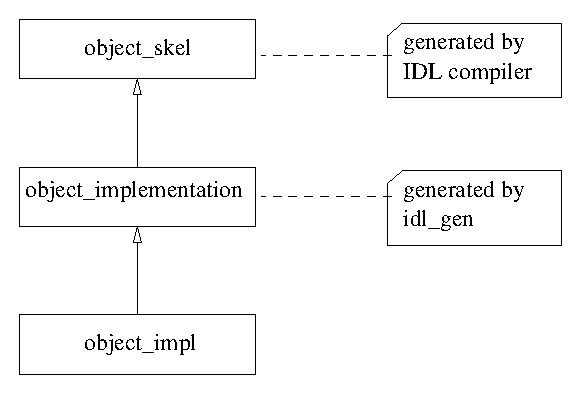
\includegraphics[height=3.8cm]{generationgap.eps}
\end{center}
\caption{\label{f_prog_generation_gap}Application of the \textsc{Generation
Gap} pattern in \qidl.}
\end{figure}

\subsubsection{\label{s_prog_singleton}Singleton and Abstract Factory}
Probably the most well-known and widely used design pattern is the
\textsc{Singleton} \cite[pp. 127-134]{b_gof}. It is used whenever there is
supposed to be only one instance of a class in one program. Singletons are
often used as an \textsc{Abstract Factory} \cite[pp. 87-95]{b_gof} as well.
These provide methods that create instances of other classes, but usually
return polymorphic subclasses.

The \texttt{Codine\_Master\_impl} class is such a combination of Singleton
and Abstract Factory. There is only one instance in the program (ensured by
the protected constructor and the \texttt{initialize()} function), and it
creates instances of other classes with its \texttt{newXXX()} methods, e.g.
\texttt{newJob()}. This is declared to return a \texttt{Codine\_Job} object,
but its implementation actually returns an object of type
\texttt{Codine\_Job\_impl}, which is 3 steps further down in the inheritance
hierarchy.

\subsubsection{Facade}
\textsc{Facade} \cite[pp. xx-yy]{b_gof} is a relatively unknown pattern. Its
purpose is to provide a simplified interface to clients that only need to
invoke one method of this interface. This in turn uses many correlated
objects in the background and possibly invokes several of their functions to
accomplish the desired task.

The \master\ interface provides a Facade to \qidl\ clients that want to
register and unregister a CORBA server that is running as a \codine\ job.
Without these functions, the client would have to retrieve the job list from
the master, find the appropriate job with its job id value and modify the
job's context attribute by appending the IOR to or deleting it from the
context list. Although not implemented yet, the \master\ object may provide
additional "shortcut" functions that perform complex, maybe even
transaction-like tasks with only one method invocation from the client.

\subsection{Tests}
\subsubsection{The Test Client}
To test the \qidl\ functionality, a simple and easily extensible test client
was developed. Its main program establishes a connection to the \qidl\
master as described in the user documentation, section
\ref{s_user_connecting}. It then evaluates the given command line arguments
and invokes a corresponding function via an array of function pointers. It is
defined as follows:

\begin{Verbatim}[fontsize=\small, frame=single]
typedef void (action_func)(Codine_Master_var master);
struct action {
   const char*   name;
   action_func*  func;
   const char*   desc;
   action(const char* n, action_func f, const char* d) :
            name(n), func(f), desc(d) {}
} actions[] = {
 action("simple", simple, "displays queues in an endless loop"),
 action("rw", readwrite, "reads and writes no. of slots of first q."),
 action("destroy", destroy, "prompts the user and destroys queues"),
 action("create", create, "prompts the user and creates a new queue"),
 action("qcplxmod", qcplxmod, "lets the user modify a q's complexes"),
 action("jobtest", jobtest, "displays jobs"),
 action("event", event, "acts as a simple event client"),
 action("doc_3", doc_sub, "the job submit example from the user doc")
};
\end{Verbatim}

Each entry in this array contains a name (the one that has to be specified in
the command line), the address of the corresponding function, and a short
description printed as a help message (shown when no argument is given). The
main program simply compares the command line argument with each of the names
from the array and calls the corresponding function to perform the desired
task. By adding a new function and an array entry, the test client can be
extended to test another feature of the \qidl\ server.

Several of these test clients, each of them running in an endless loop, in
addition to some conventional \codapi\ clients were run concurrently to
provoke race conditions and make load tests. Apart from producing serious
Linux/Alpha kernel crashes, they posed no problem to \qidl.

\subsubsection{JQmon}
Another important test facility was the Java version of Qmon. Its first
prototype was developed as part of a diploma thesis, using the C \codapi\ via
the Java Native Interface. This was replaced by CORBA by a Rumanian
guest student, Laurentiu Petrea, taking part in a European program.
JQmon was actually the first "real"
application to use \qidl, especially as an event client. This evaluated and
improved the event handling facility of \qidl, and---of course---surfaced
several bugs in the code.

\subsection{\label{s_prog_extending}Extending the Server}
This last section shows how easy it is to extend the \qidl\ server. The 
main ways of doing so is to

\begin{itemize}
\item add convenience functions
\item add new cull list elements to existing objects
\item add new objects
\end{itemize}

The first one is relatively easy. Just adding a method to the object's IDL
interface (between \texttt{/*IDL} and \texttt{XIDL*/}) in the api header
file, and implementing the function in the \texttt{\_impl} class is all there
is to do. Then it's only using the objects in a more or less intelligent way.

Adding new list elements is even easier if it is only a fundamental data type
or a struct---simply recompile \qidl! If the new element references another
object, you'll only have to write the \texttt{get\_} and \texttt{set\_}
methods. Usually, this is not very complicated as well.

Adding new objects like a queue or a job is a bit more work, although this
follows a common pattern applied to all other objects, too. There are several
steps to do.

\begin{enumerate}
\item Write the object's cull list in a (possibly new) api header file.
\item Append the object to the \texttt{OBJECTS} variable in the \qidl\
makefile. If it is in a new header file, don't forget to append the file to
the \texttt{IDLSRC} variable.
\item Write the object's implementation (see section
\ref{s_prog_server_objects}) in the \texttt{\_impl.h} and \texttt{\_impl.cpp}
files.
\item Extend the \master\ interface with the \texttt{getXXX()} and
\texttt{newXXX()} functions.
\item Extend the \texttt{Codine\_Master\_impl} class:
   \begin{enumerate}
   \item implement the new functions from the IDL interface.
   \item append a data member containing the list of object references.
   \item initialize the list in the \texttt{initialize()} method.
   \item provide the internal \texttt{getXXX()} and \texttt{getXXXImpl()}
   functions.
   \item extend the \texttt{addObject()} and \texttt{deleteObject()}
   functions to handle the new object type.
   \end{enumerate}
\item Write a new \texttt{object\_changed()} function in the 
\texttt{qidl\_c\_api} files and invoke this from somewhere in the \codine\ 
kernel code. This is usually done in the \texttt{cod\_add\_list\_event\_}
function.
\end{enumerate}


\cleardoublepage
\section{Conclusion and Final Remarks}
\subsection{The \qidl\ Project}
\subsubsection{Migrating to New Technologies}
\qidl\ introduced a whole lot of new technologies to \codine: C++, STL,
multithreading, CORBA---and was successful. There were serious doubts about
the stability of the product, especially concerning the subtle implications
of multithreading. Yet it turned out to be a robust product, admittedly after
a lot and hard work of in-depth debugging.

A first test as part of the \textsc{Autobench} project funded by the 
German ministry for education and research (BMBF) was successfully
accomplished. Part of \qidl's functionality was used in a production-like
environment in the automobile industry. This demonstration proved once again,
that the advance in technology was a courageous, but worthwhile step into
\codine's future.

\subsubsection{Things to Be Done}
Most important in this respect is certainly testing. It is almost impossible 
to test the full range of \qidl\
functionality in all thinkable variations. Especially the concurrent use of
\codapi\ and \qidl\ with its inherent race conditions opens traps and pitfalls
that may appear only in very special and non-reproduceable occasions---or
never at all! These and other hidden faults in the program can probably only
be discovered by productive use of \qidl\ by first pilot customers. Hopefully
by the end of this year, BMW will be the first commercial customer
to have \qidl\ installed in their engineering center in Munich.

Providing \qidl\ to customers will surely open another field for extensions:
convenience functions. There are only very few of those implemented so far
(see section \ref{s_user_convenience}), but the \qidl\ design is flexible
enough to cope with an increased demand in easy-to-use or "short-cut"
methods.

The last future aim is to port \qidl\ to other platforms. Currently it is
running on:
\begin{itemize}
\item Linux/Intel
\item Linux/Alpha (unstable due to kernel problems)
\item DEC OSF4
\item IRIX 6.5
\item Solaris 7/Intel
\end{itemize}
The actual porting effort is really not worth mentioning since \qidl\ was
programmed adhering to all possible standards. But the prerequisites are
difficult to come by on many platforms:
\begin{itemize}
\item ANSI C++ compiler (namespaces, exception handling, STL)
\item POSIX threads library
\item ORBacus availability
\item lex/yacc available and working in conjunction with C++
\end{itemize}
Once these requirements have been met, a simple call to \texttt{make} is
usually all there is to do to get \qidl\ running.

\subsection{Genias---The Company}
Last but not least, some words about Genias. I enjoyed working in the company
very much, with a young team of employees who helped me willingly at any time.
Being offered a cluster of 23 UNIX
workstations of all kinds---from AIX to Solaris, and Alpha to Sparc---far away
from the everyday Microsoft-Intel-PC world, one can experience a whole new
way of working and become accustomed to a still dominating operating system
in the scientific world.

My participation in two public projects (\textsc{Autobench} from BMBF, and
\textsc{Julius}, an EU-sponsored ESPRIT project) brought me to meetings and
conferences in Munich and St. Augustin, the first one in an international
environment with partners from all over Europe, where I had a chance to
present my work.

All in all, I can recommend an internship at Genias for any student who
\begin{itemize}
\item is willing to leave behind his or her PC
\item can do without an integrated development environment (IDE)
\item wants to learn---and give---a lot.
\end{itemize}

\newpage
\nocite{*}
\bibliographystyle{alpha}
\bibliography{manual}

\end{document}
